\documentclass[a4paper, 10pt, ]{article}

\usepackage[slovak]{babel}





\usepackage[utf8]{inputenc}
\usepackage[T1]{fontenc}

\usepackage[left=4cm,
			right=4cm,
            % left=2.5cm,
			% right=5.5cm,
			top=2.1cm,
			bottom=2.6cm,
			footskip=7.5mm,
			% twoside,
			marginparwidth=3.0cm,
			%showframe,
			]{geometry}

\usepackage{graphicx}
\usepackage[dvipsnames]{xcolor}
% https://en.wikibooks.org/wiki/LaTeX/Colors


% ------------------------------

\usepackage{lmodern}

\usepackage[tt={oldstyle=false,proportional=true,monowidth}]{cfr-lm}

% ------------------------------

\usepackage{amsmath}
\usepackage{amssymb}
\usepackage{amsthm}

\usepackage{booktabs}
\usepackage{multirow}
\usepackage{array}
\usepackage{dcolumn}


\usepackage[singlelinecheck=true]{subfig}


% ------------------------------


\def\naT{\mathsf{T}}

\hyphenpenalty=6000
\tolerance=1000




% ------------------------------


\makeatletter

	\def\@seccntformat#1{\protect\makebox[0pt][r]{\csname the#1\endcsname\hspace{4mm}}}

	\def\cleardoublepage{\clearpage\if@twoside \ifodd\c@page\else
	\hbox{}
	\vspace*{\fill}
	\begin{center}
	\phantom{}
	\end{center}
	\vspace{\fill}
	\thispagestyle{empty}
	\newpage
	\if@twocolumn\hbox{}\newpage\fi\fi\fi}

	\newcommand\figcaption{\def\@captype{figure}\caption}
	\newcommand\tabcaption{\def\@captype{table}\caption}

\makeatother


% ------------------------------




\usepackage{fancyhdr}
\fancypagestyle{plain}{%
\fancyhf{} % clear all header and footer fields
\fancyfoot[C]{\sffamily {\bfseries \thepage}\ | {\scriptsize\oznacenieCasti}}
\renewcommand{\headrulewidth}{0pt}
\renewcommand{\footrulewidth}{0pt}}
\pagestyle{plain}


% ------------------------------


\usepackage{titlesec}
\titleformat{\paragraph}[hang]{\sffamily  \bfseries}{}{0pt}{}
\titlespacing*{\paragraph}{0mm}{3mm}{1mm}
\titlespacing*{\subparagraph}{0mm}{3mm}{1mm}

\titleformat*{\section}{\sffamily\Large\bfseries}
\titleformat*{\subsection}{\sffamily\large\bfseries}
\titleformat*{\subsubsection}{\sffamily\normalsize\bfseries}






% ------------------------------

\PassOptionsToPackage{hyphens}{url}
\usepackage[pdfauthor={},
			pdftitle={},
			pdfsubject={},
			pdfkeywords={},
			% hidelinks,
			colorlinks=false,
			breaklinks,
			]{hyperref}


% ------------------------------


\graphicspath{%
{../fig_standalone/}%
{../../PY/fig/}%
{../../PY/jupynotex/fig/}%
{../../ML/fig/}%
{./fig/}%
}



% ------------------------------

\usepackage{enumitem}

\usepackage{lettrine}

% ------------------------------


\usepackage{microtype}


% ------------------------------

\usepackage[titles]{tocloft}

\setlength{\cftsecindent}{-12mm}
\setlength{\cftsecnumwidth}{12mm}
\renewcommand{\cftsecpresnum}{\hfill}
\renewcommand{\cftsecaftersnum}{\hspace{4mm}}

\setlength{\cftsubsecindent}{-12mm}
\setlength{\cftsubsecnumwidth}{16mm} % 12 + 4
\renewcommand{\cftsubsecpresnum}{\hfill}
\renewcommand{\cftsubsecaftersnum}{\hspace{8mm}} % 4 + 4 mm

\setlength{\cftsubsubsecindent}{-12mm}
\setlength{\cftsubsubsecnumwidth}{20mm} % 12 + 4 + 4
\renewcommand{\cftsubsubsecpresnum}{\hfill}
\renewcommand{\cftsubsubsecaftersnum}{\hspace{12mm}} % 4 + 4 + 4 mm

\renewcommand{\cftsecpagefont}{\lstyle \bfseries}
\renewcommand{\cftsubsecpagefont}{\lstyle}
\renewcommand{\cftsubsubsecpagefont}{\lstyle}



\setlength{\cftparaindent}{-16mm}
\setlength{\cftparanumwidth}{28mm} % 16 + 4 + 4 + 4
\renewcommand{\cftparapresnum}{\hfill}
\renewcommand{\cftparaaftersnum}{\hspace{16mm}} % 4 + 4 + 4 + 4 mm








% ------------------------------

\usepackage{listings}



\renewcommand{\lstlistingname}{Výpis kódu}
\renewcommand{\lstlistlistingname}{Výpisy kódu}




%New colors defined below
\definecolor{codegreen}{rgb}{0,0.6,0}
\definecolor{codegray}{rgb}{0.5,0.5,0.5}
\definecolor{codepurple}{rgb}{0.58,0,0.82}
\definecolor{backcolour}{rgb}{0.95,0.95,0.95}

%Code listing style named "mystyle"
\lstdefinestyle{mystyle}{
  backgroundcolor=\color{backcolour},
  commentstyle=\fontfamily{lmtt}\fontsize{8.5pt}{8.75pt}\selectfont\color{codegreen},
  keywordstyle=\fontfamily{lmtt}\fontsize{8.5pt}{8.75pt}\selectfont\bfseries\color{Blue},
  stringstyle=\fontfamily{lmtt}\fontsize{8.5pt}{8.75pt}\selectfont\color{codepurple},
  basicstyle=\fontfamily{lmtt}\fontsize{8.5pt}{8.75pt}\selectfont,
  breakatwhitespace=false,
  breaklines=true,
  captionpos=t,
  keepspaces=true,
  numbers=left,
  numbersep=4mm,
  numberstyle=\fontfamily{lmtt}\fontsize{8.5pt}{8.75pt}\selectfont\color{lightgray},
  showspaces=false,
  showstringspaces=false,
  showtabs=false,
  tabsize=2,
  % xleftmargin=10pt,
  framesep=10pt,
  language=Python,
  escapechar=|,
}


\lstset{
    inputencoding=utf8,
    extendedchars=true,
    literate=%
    {á}{{\'a}}1
    {č}{{\v{c}}}1
    {ď}{{\v{d}}}1
    {é}{{\'e}}1
    {ě}{{\v{e}}}1
    {í}{{\'i}}1
    {ň}{{\v{n}}}1
    {ó}{{\'o}}1
    {ř}{{\v{r}}}1
    {š}{{\v{s}}}1
    {ť}{{\v{t}}}1
    {ú}{{\'u}}1
    {ů}{{\r{u}}}1
    {ý}{{\'y}}1
    {ž}{{\v{z}}}1
    {Á}{{\'A}}1
    {Č}{{\v{C}}}1
    {Ď}{{\v{D}}}1
    {É}{{\'E}}1
    {Ě}{{\v{E}}}1
    {Í}{{\'I}}1
    {Ň}{{\v{N}}}1
    {Ó}{{\'O}}1
    {Ř}{{\v{R}}}1
    {Š}{{\v{S}}}1
    {Ť}{{\v{T}}}1
    {Ú}{{\'U}}1
    {Ů}{{\r{U}}}1
    {Ý}{{\'Y}}1
    {Ž}{{\v{Z}}}1
    {ô}{{\^{o}}}1
}


% ------------------------------


\usepackage{caption}

\DeclareCaptionFormat{odsadene}{\protect\makebox[0pt][r]{#1#2\hspace{4mm}}#3\par}
\DeclareCaptionLabelSeparator{lendvojbodka}{:}
% \DeclareCaptionFont{lightgray}{\color{lightgray}}
\DeclareCaptionFont{lightgray}{\fontfamily{lmtt}\fontsize{8.5pt}{8.75pt}\selectfont\color{lightgray}}

\captionsetup[lstlisting]{format=odsadene, labelsep=lendvojbodka, justification=raggedright, singlelinecheck=false, labelfont={sf, lightgray},}


% ------------------------------





% ------------------------------

\usepackage[backend=biber,
            style=numeric,
            sorting=none,
            ]{biblatex}
\DeclareSourcemap{
    \maps[datatype=bibtex]{
        \map{
        \step[fieldset=note, null]
        }
        \map{
        \step[fieldset=file, null]
        }        
        % \map{
        % \step[fieldset=url, null]        
        % }
        \map{
        \step[fieldset=eprint, null]
        }
    }
}


\addbibresource{E:/_CurrentContent/01_work_repo/bibLaTeXDB/bibLaTeXDB.bib} % nonpublic data





\def\oznacenieCasti{MRS09 - ZS2024}


\usepackage{longtable}




\begin{document}


\lstset{%
style=mystyle,
rangebeginprefix=\#\#\#\ cellB\ ,%
rangebeginsuffix=\ \#\#\#,%
rangeendprefix=\#\#\#\ cellE\ ,%
rangeendsuffix=\ \#\#\#,%
includerangemarker=false,
}





\fontsize{12pt}{22pt}\selectfont

\centerline{\textsf{Modelovanie a riadenie systémov} \hfill \textsf{\oznacenieCasti}}

\fontsize{18pt}{22pt}\selectfont





\begin{flushleft}
	\textbf{\textsf{Vybrané charakteristiky dynamického systému}}
\end{flushleft}





\normalsize

\bigskip

{\hypersetup{hidelinks}

\tableofcontents

}

\bigskip

\vspace{18pt}



\noindent
\lettrine[lines=3, nindent=0pt]{H}{lavnou} témou tohto textu sú \emph{prevodová charakteristika} a \emph{prechodová charakteristika} dynamického systému. Uvažuje sa systém, ktorý má jeden vstupný signál $u(t)$ a jeden výstupný signál $y(t)$ a~tieto sú spojité v čase a dynamický systém je časovo invariantný.



% Pojem \emph{rád systému} má v podstate rovnaký význam ako pri diferenciálnej rovnici. Diferenciálna rovnica $n$-tého rádu opisuje dynamický systém $n$-tého rádu. Dif. rovnica $n$-tého rádu je taká, v ktorej vystupuje maximálne $n$-tá derivácia neznámej. V kontexte prenosovej funkcie systému to znamená, že charakteristický polynóm systému je $n$-tého stupňa.

% Osobitne uvedieme, že samozrejme uvažujeme \emph{kauzálny systém}, teda výstup systému je následkom diania v súčastnosti a minulosti. Z matematického hľadiska na prenosovú funkciu to znamená, že pre stupne polynómov $A(s)$ a $B(s)$ platí $n \geq m$ pričom charakteristický polynóm $A(s)$ má stupeň $n$, polynóm $B(s)$ má stupeň $m$ a uvažujme prenosovú funkciu v tvare
% \begin{equation}
%     G(s) = \frac{B(s)}{A(s)}
% \end{equation}






\section{O ustálenom stave systému}

Pri skúmaní vlastností systému je často ako prvé potrebné poznať tzv. statické vlastnosti systému. Vo všeobecnosti sa to týka ustálených stavov systému. Typickým príkladom je situácia, keď vstupný signál $u(t)$ je konštantný, jeho hodnota sa nemení v čase. Ustálenú hodnotu vstupného signálu označme $u(\infty)$, čím sa zdôrazňuje, že ide o hodnotu akoby v čase nekonečno, čo v praxi je čas taký, keď všetky prechodné deje považujeme za skončené. Otázkou je, či sa aj hodnota výstupného signálu $y(t)$ ustáli na nejakej hodnote $y(\infty)$. 

Na prvý pohľad je zrejmé, že naznačené statické vlastnosti systému nemá zmysel skúmať pre systém, ktorý je nestabilný.



\paragraph{Stabilita systému}

Pod pomenovanim \emph{stabilita systému} sa typicky rozumie niekoľko rôznych prípadov týkajúcich sa všeobecného riešenia diferenciálnej rovnice opisujúcej dynamický systém. Intuitívnym je termín \emph{BIBO stabilita} (bounded input, bounded output), kde sa skúma prípad, keď vstupný signál $u(t)$ je ohraničený, jeho max. hodnota je menej ako nekonečno. Ak je potom výstupný signál $y(t)$ tiež ohraničený, hovoríme, že systém je BIBO stabilný. V podstate sa tak skúma vnútená zložka riešenia nehomogénnej diferenciálnej rovnice. Vlastnú zložku riešenia, závislú od začiatočných podmienok, je možné skúmať rovnako a súvisí to s pojmom \emph{asymptotická stabilita}. 

\smallskip

Pri lineárnom systéme systéme platí, že vlastnosti systému z akéhokoľvek hľadiska stability sú kompletne určené pólmi systému, teda koreňmi charakteristického polynómu. Nutnou a postačujúcou podmienkou stability lineárneho systému je, aby všetky póly systému ležali v ľavej polrovine komplexnej roviny, t.j. aby ich reálne časti boli záporné. Ak aspoň jeden pól leží na imaginárnej osi, hovoríme, že systém je na hranici stability. Ak je aspoň jeden pól v pravej polrovine, jeho reálna časť je kladná, hovoríme, že systém je nestabilný.




\paragraph{Statické zosilnenie verzus astatizmus}

Uvažujme systém, ktorý nie je nestabilný. Z hľadiska statických vlastností systému je možné rozlišovať dve základné vlastnosti, ktoré súvisia s ustáleným stavom systému. Prvou je \emph{statické zosilnenie} systému, druhou je \emph{astatizmus} systému.

Ak je vstupný signál $u(t)$ konštantný, jeho hodnota je $u(\infty)$, a výstupný signál $y(t)$ sa ustáli na hodnote $y(\infty)$, potom hovoríme, že systém je v ustálenom stave. Je možné určiť statické zosilnenie systému, ktoré je pomer ustálenej hodnoty výstupného signálu k ustálenej hodnote vstupného signálu.

Ak je vstupný signál $u(t)$ konštantný, jeho hodnota je $u(\infty)$, a výstupný signál $y(t)$ sa neustáli, neprestane sa meniť, neprestane rásť, hovoríme o astatizme systému, systém je astatický, neustáli sa.


\smallskip

Pri lineárnom systéme ak žiadny z pólov systému nie je nulový, potom systému dávame prívlastok statický. Stále však máme na mysli dynamický systém, ktorý ja daný napríklad prenosovou funkciou systému. Pre takýto systém je možné určiť jeho statické zosilnenie. Statické zosilnenie je pomer výstupu ku vstupu v ustálenom stave. Ak je jeden z pólov systému nulový, hovoríme, že systém je astatický („obsahuje astatizmus“). Ak práve jeden pól je nulový, hovoríme o astatizme prvého rádu (ak dva póly, potom astatizmus druhého rádu, atď). Pripomeňme, že uvažujeme systém, ktorý nie je nestabilný. Nulový pól znamená, samozrejme, že jeho reálna časť je nulová. Z~hľadiska stability to znamená, že systém je na hranici stability.


\paragraph{Prevodová charakteristika}

V kontexte statických vlastností systému má vo všeobecnosti význam hovoriť o~prevodovej charakteristike systému. Prevodová charakteristika je závislosť ustálených hodnôt výstupného signálu systému od ustálených hodnôt vstupného signálu systému.

Je zrejmé, že prevodová charakteristika sa týka systémov s prívlastkom statické, teda takých, ktoré nie sú astatické.

\smallskip

V prípade lineárnych systémov je prevodová charakteristika priamka a bez straty na všeobecnosti môžeme uvažovať, že prechádza začiatkom súradnicového systému. Sklon priamky je daný statickým zosilnením systému.







\section{O meraní prevodovej charakteristiky}


Prevodová charakteristika je závislosť ustálených hodnôt výstupnej veličiny od ustálených hodnôt vstupnej veličiny. Prevodová charakteristika, niekde sa nazýva aj statická charakteristika, teda charakterizuje systém len v~ustálených stavoch. Neobsahuje informáciu o dynamike systému.


\paragraph{Simulovaný systém}

V nasledujúcom sa pokúsime načrtnúť meranie prevodovej charakteristiky. Tu sa však nebude naozaj niečo merať, ale reálny systém bude nahradený simulovaným. Proces získavania „surových“ dát, ktoré sú potrebné pre určenie prevodovej charakteristiky a~proces spracovania týchto dát bude však rovnaký akoby išlo o reálny systém.


Systém, ktorý bude predmetom skúmania, ktorého prevodovú charakteristiku budeme merať, je kyvadlo, tak ako bolo už skôr opísané. Navyše však bude k výstupnej veličine simulovaného systému pridaný čitateľovi neznámy šum. Dôvodom je lepšie napodobenie situácie v akej by bol čitateľ ak by sa zaoberal výstupnou veličinou reálneho systému.

Pripomeňme, že uvažujme kyvadlo, ktorého kmity sú tlmené viskóznym trením s~koeficientom $\beta$ [kg~m$^2$~s$^{-1}$]. Kyvadlo je na Obr.~\ref{Kyvadlo}, kde hmotný bod s~hmotnosťou $m$ [kg] pripevnený na ramene so zanedbateľnou hmotnosťou a~dĺžkou $l$ [m] kmitá, $o$~označuje os otáčania kolmú na rovinu, v~ktorej kyvadlo kmitá, uhol medzi zvislicou a~ramenom kyvadla je označený $\varphi$ [rad] a~gravitačné zrýchlenie $g$~[m~s$^{-2}$].
\begin{center}

    \vbox{%
	\makebox[\textwidth][c]{%
	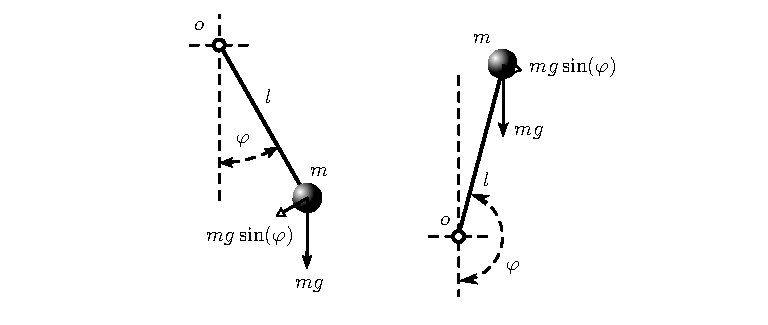
\includegraphics{Obr_Kyvadlo.pdf}
	}
	\vspace{-9mm}

	\figcaption{Kyvadlo}
	\label{Kyvadlo}
    }

	\vspace{-3mm}
\end{center}
Pohybová rovnica opisujúca dynamiku rotačného pohybu kyvadla môže byť v tvare
\begin{align}
	\ddot{\varphi}(t) = - \frac{\beta}{ml^2} \dot{\varphi}(t) - \frac{g}{l} \sin\left(\varphi(t)\right) + \frac{1}{ml^2}u(t)
\end{align}
kde $u(t)$ [kg~m$^2$~s$^{-2}$] je externý moment sily pôsobiaci na rameno kyvadla, $\dot{\varphi}(t)$ [rad~s$^{-1}$] je uhlová rýchlosť a~$\ddot{\varphi}(t)$~[rad~s$^{-2}$] je uhlové zrýchlenie ramena kyvadla. Číselné hodnoty parametrov kyvadla sú uvedené v tabuľke~\ref{Parametre kyvadla}.
\begin{center}

    \vbox{
    
    \tabcaption{Parametre kyvadla}
    \label{Parametre kyvadla}
    
    \vspace{-3mm}
    
    \begin{tabular*}{\textwidth}{ c @{\extracolsep{\fill}} c c}
        
        \toprule
        Parameter   & Hodnota    & Jednotky              \\
        \midrule
            $m$       & $1$   & kg             \\
            $l$    &  $1$  & m \\
            $g$   & $9,81$  & m s$^{-2}$ \\
            $\beta$  &  $2\ \sqrt{g/l}$ &  kg~m$^2$~s$^{-1}$ \\
        \bottomrule\
    
    \end{tabular*}
    } 
    
    \vspace{-3mm}
    
\end{center}


\subsection{Dáta pre určenie prevodovej charakteristiky}

Ako už bolo uvedené, predmetom záujmu sú ustálené hodnoty výstupného signálu. Ak na vstup privedieme vstupný signál s nejakou konštantnou vstupnou hodnotou, následne počkáme istý čas nech sa výstupný signál ustáli, tak potom môžeme odčítať (odmerať) ustálenú hodnotu výstupného signálu. Takto sa získa jeden bod z prevodovej charakteristiky.

Hneď potom je však možné zmeniť hodnotu vstupného signálu a opäť čakať, kým sa výstup ustáli.

Tento postup, hodnoty vstupného signálu a doby, počas ktorých sa „čaká“ na ustálenie výstupu, možno vyjadriť tabuľkou nasledovne. Prvý stĺpec je čas, v ktorom sa zmení (prepne) vstup a druhý stĺpec je hodnota (konštanta), na ktorú sa zmení (prepne).
\begin{center}

    \vbox{
    
    \tabcaption{Hodnoty vstupného signálu}
    \label{Hodnoty vstupného signálu}
    
    % \vspace{-3mm}
    
    \begin{tabular}{     c      c       }
        \toprule
        čas [s] & hodnota [kg m$^2$ s$^{-2}$] \\
        \midrule
        $0$ & $0,0$ \\
        $10$ & $1,0$ \\
        $30$ & $2,0$ \\
        $20$ & $3,0$ \\
        $40$ & $4,0$ \\
        $50$ & $5,0$ \\
        $60$ & $6,0$ \\
        $70$ & $7,0$ \\
        $80$ & $8,0$ \\
        $95$ & $9,0$ \\
        $110$ & $9,5$ \\
        $135$ & $9,81$ \\
        \bottomrule
        \end{tabular}
    } 
    
    % \vspace{-3mm}
    
\end{center}
Z uvedeného je zároveň jasné, že interval vstupných hodnôt, pre ktorý zisťujeme ustálené hodnoty výstupu je $0$ až $9,81$ [kg m$^2$ s$^{-2}$]. Iné by vzhľadom na konkrétne kyvadlo, ktoré sa tu uvažuje, malo pramalý význam.

Vstupný signál tak ako je definovaný tabuľkou~\ref{Hodnoty vstupného signálu} možno znázorniť ako na obr.~\ref{MRS09_figsc_01_1}.
\begin{center}

    \vbox{%
	\makebox[\textwidth][c]{%
	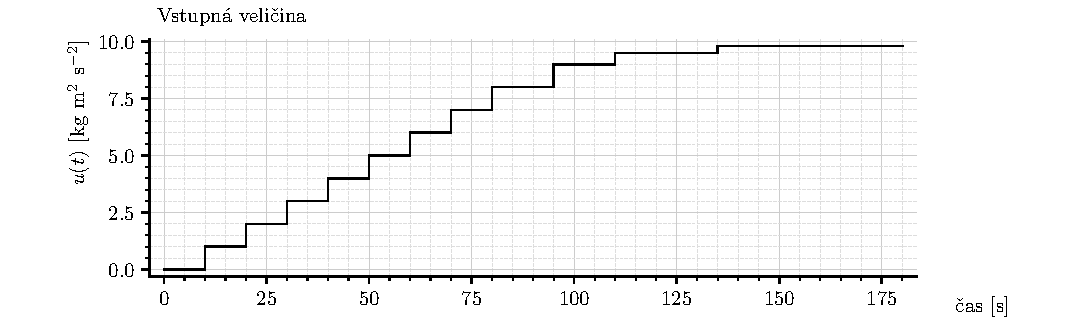
\includegraphics{MRS09_figsc_01_1.pdf}
	}

    \vspace{-6pt}

	\figcaption{Priebeh vstupného signálu}
	\label{MRS09_figsc_01_1}
    }

\end{center}

Simulujme teraz priebeh výstupnej veličiny kyvadla (výchylky kyvadla) pri uvedenom vstupnom signály. Výsledok je na obr.~\ref{Surové dáta}.
\begin{center}

    \vbox{%
	\makebox[\textwidth][c]{%
	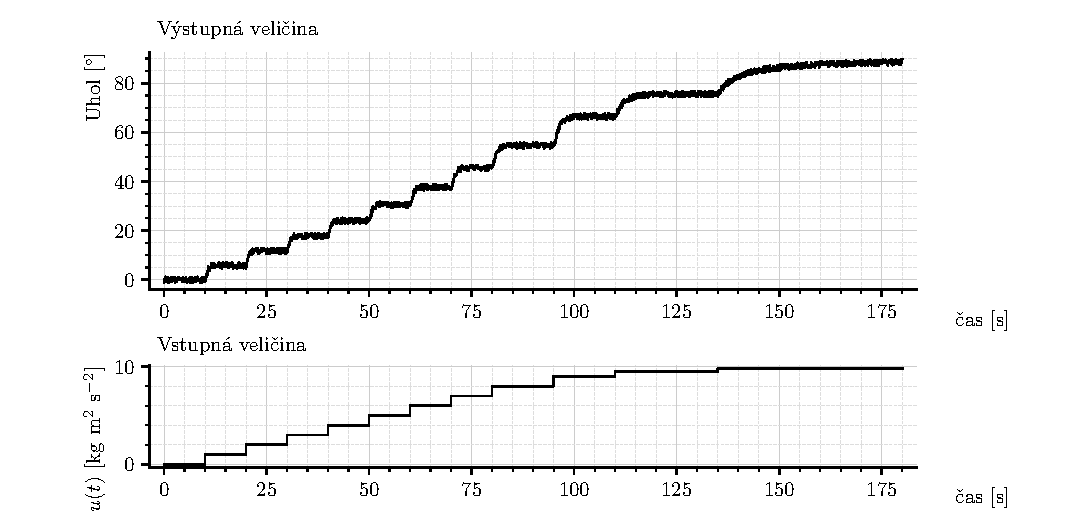
\includegraphics{MRS09_figsc_02_2.pdf}
	}

    \vspace{-6pt}

	\figcaption{Surové dáta. Poznámka: výstupná veličina na obr.~\ref{Surové dáta} je schválne „zašumená“. Napodobňujeme tu tým potenciálny šum snímača, ktorý meria danú veličinu. Dôvodom je najmä skutočnosť, že sa tak lepšie ilustrujú jednotlivé kroky potrebné pre všeobecné spracovanie nameraného signálu, ktoré sú uvedené v ďalších častiach.}
	\label{Surové dáta}
    }

\end{center}




\subsection[Spracovanie dát]{Spracovanie dát}

Zo surových dát je potrebné získať jednotlivé body prevodovej charakteristiky. To v~prvom rade znamená byť schopný odčítať ustálenú hodnotu výstupného signálu (zo surových dát). Pre ilustráciu, venujme sa nameraným dátam od desiatej sekundy po dvadsiatu sekundu, teda pre interval, počas ktorého bola na vstupe hodnota $u=1$ [kg m$^2$ s$^{-2}$]. Táto časť dát je nakreslená na obr.~\ref{Surové dáta - detail}.
\begin{center}

    \vbox{%
    \makebox[\textwidth][c]{%
    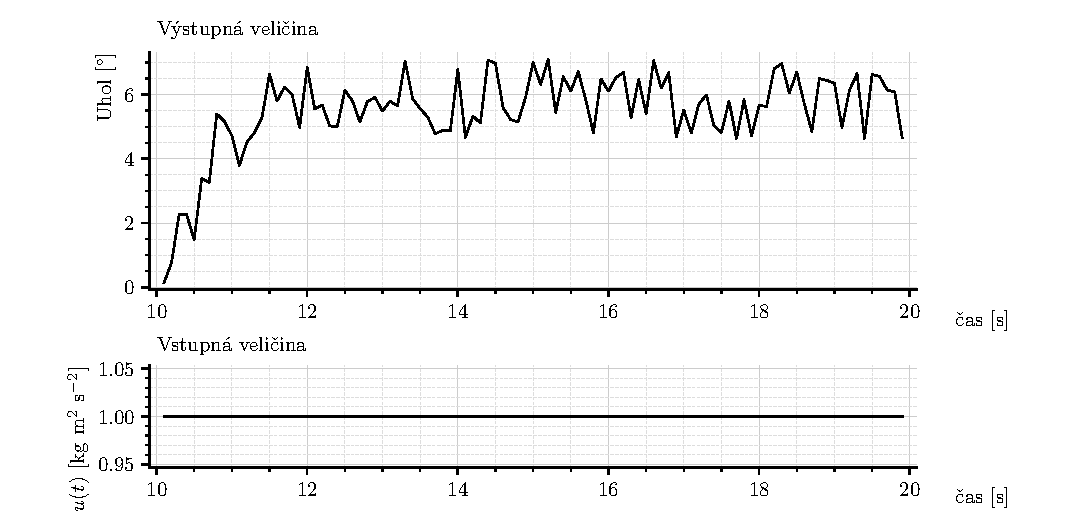
\includegraphics{MRS09_figsc_03_3.pdf}
    }

    \vspace{-6pt}

    \figcaption{Surové dáta - detail}
    \label{Surové dáta - detail}
    }

\end{center}
Z obr.~\ref{Surové dáta - detail} je zrejmé, že v poslednej tretine intervalu je už možné považovať hodnotu výstupu za ustálenú. Vyznačme túto časť dát - viď obr.~\ref{Surové dáta - detail2}.
\begin{center}

    \vbox{%
    \makebox[\textwidth][c]{%
    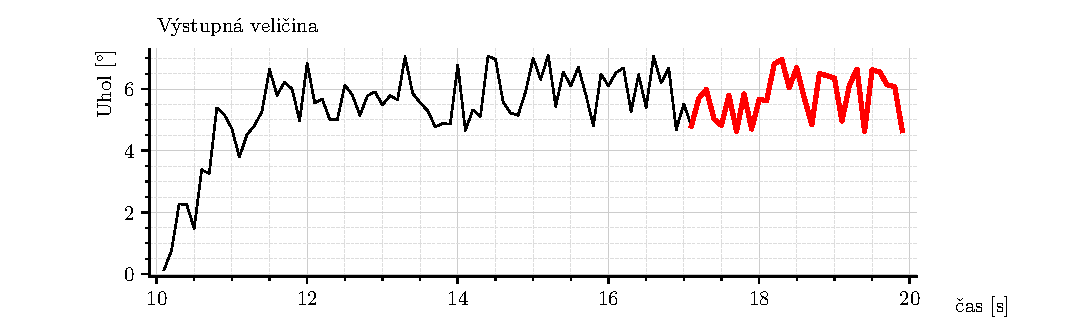
\includegraphics{MRS09_figsc_04_4.pdf}
    }

    \vspace{-6pt}

    \figcaption{Surové dáta - detail}
    \label{Surové dáta - detail2}
    }

\end{center}
Otázka je, ako z vyznačeného úseku určiť jednu hodnotu - ustálenú hodnotu. Prirodzenou voľbou je urobiť priemer z vybranej (vyznačenej) časti dát. Priemer je vyznačený na obr.~\ref{Surové dáta - detail3}
\begin{center}

    \vbox{%
    \makebox[\textwidth][c]{%
    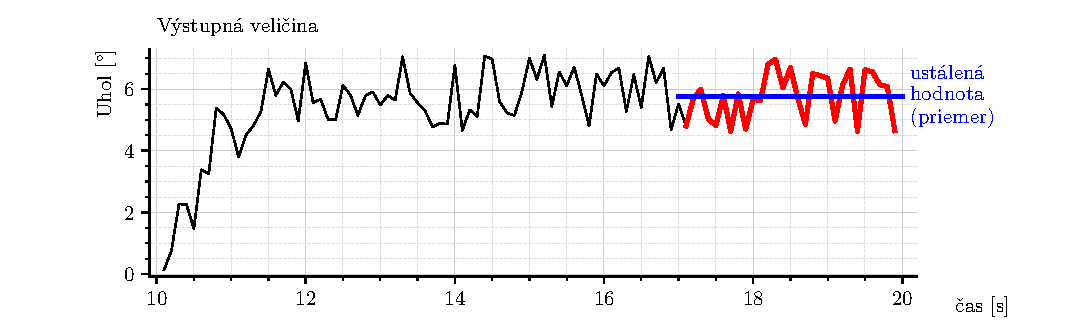
\includegraphics{MRS09_figsc_05_5.pdf}
    }

    \vspace{-6pt}

    \figcaption{Surové dáta - detail}
    \label{Surové dáta - detail3}
    }

\end{center}
Rovnako je samozrejme možné postupovať pri všetkých bodoch prevodovej charakteristiky. Všetky ustálené hodnoty odčítané zo „surových dát“ sú znázornené na obr.~ \ref{Surové dáta2}.
\begin{center}

    \vbox{%
    \makebox[\textwidth][c]{%
    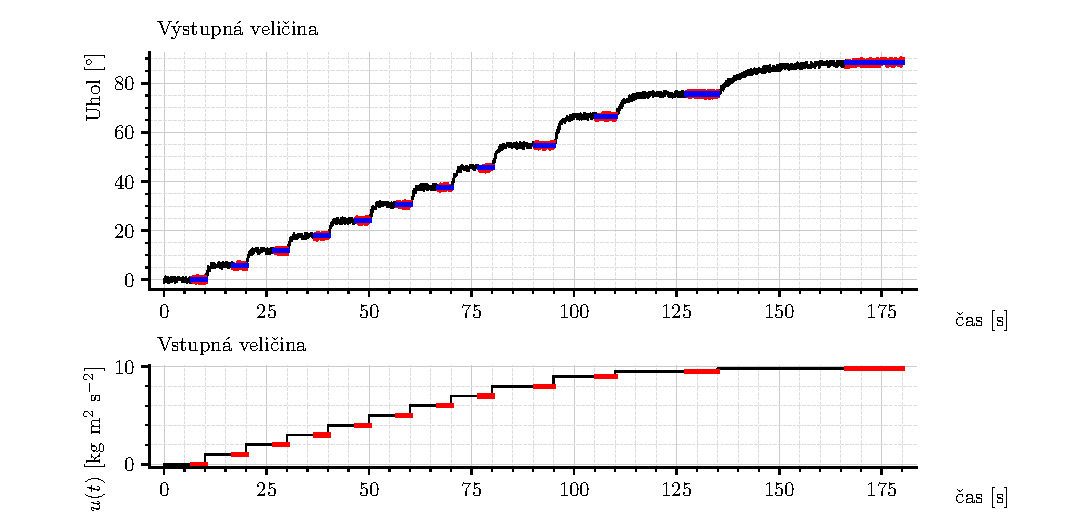
\includegraphics{MRS09_figsc_06_6.pdf}
    }

    \vspace{-6pt}

    \figcaption{Surové dáta}
    \label{Surové dáta2}
    }

\end{center}
Odčítané hodnoty sú následne uvedené v tabuľke~\ref{Prevodová charakteristika}. Prevodová charakteristika je graficky znázornená na obr.~\ref{Prevodová charakteristika graf}.
\begin{center}

    \vbox{
    
    \tabcaption{Prevodová charakteristika}
    \label{Prevodová charakteristika}
    
    % \vspace{-3mm}
    
    \begin{tabular}{     c      c       }
        \toprule
        vstup [kg m$^2$ s$^{-2}$] & výstup [°] \\
        \midrule
        $0,0$ & $0,00691$\\
        $1,0$ & $5,7$\\
        $2,0$ & $11,8$\\
        $3,0$ & $17,7$\\
        $4,0$ & $24,3$\\
        $5,0$ & $30,6$\\
        $6,0$ & $37,6$\\
        $7,0$ & $45,2$\\
        $8,0$ & $54,5$\\
        $9,0$ & $66,5$\\
        $9,5$ & $75,6$\\
        $9,81$ & $88,7$\\
        \bottomrule
        \end{tabular}
    } 
    
    % \vspace{-3mm}
    
\end{center}
\begin{center}

    \vbox{%
    \makebox[\textwidth][c]{%
    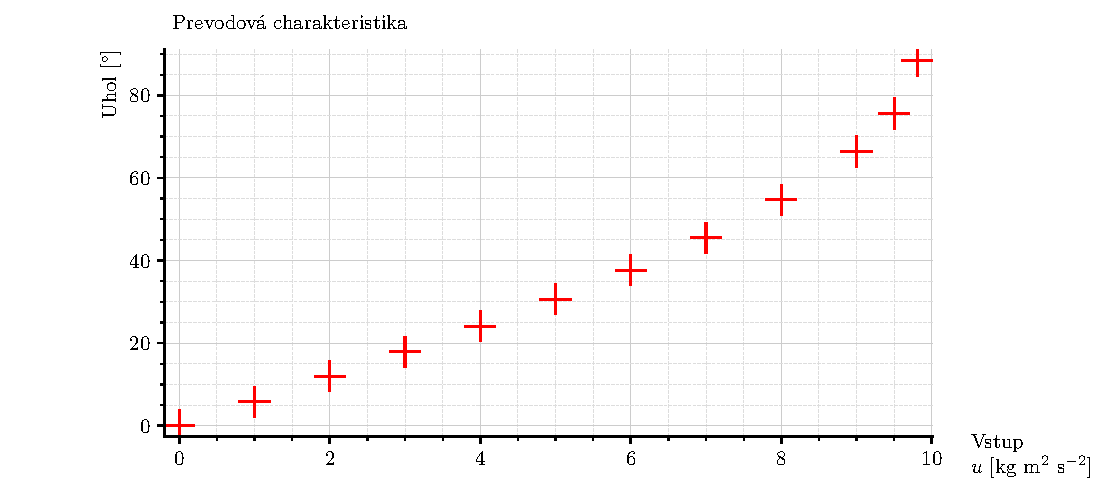
\includegraphics{MRS09_figsc_07_7.pdf}
    }

    \vspace{-6pt}

    \figcaption{Prevodová charakteristika}
    \label{Prevodová charakteristika graf}
    }

\end{center}


\subsection{Doplnkový text: o aproximácii prevodovej charakteristiky}

Majme nameranú prevodovú charakteristiku, dáta sú v tabuľke~\ref{Prevodová charakteristika}. Prevodová charakteristika je graficky znázornená na obr.~\ref{Prevodová charakteristika graf}.

Body prevodovej charakteristiky zodpovedajú istej vlastnosti reálneho systému (reálne existujúceho systému). Zodpovedajú závislosti výstupu systému od vstupu systému, samozrejme v ustálenom stave. Nameraných je však len niekoľko bodov. V týchto bodoch je daná vlastnosť systému známa. Čo však v prípade ak by bolo potrebné poznať danú vlastnosť mimo nameraných bodov? Teda mimo hodnôt vstupu, pre ktoré bola prevodová charakteristika nameraná.

Aj pre tieto účely je výhodné využiť model. Model reálnej vlastnosti systému. Samotnej vlastnosti systému zodpovedá nameraná závislosť (prevodová charakteristika). Aproximáciou tejto závislosti je možné získať model.

Model nech je v tomto prípade matematický vzťah, funkčná závislosť, istý predpis. Ak hodnota na vstupe modelu bude rovnaká ako hodnota na vstupe reálneho systému, potom hodnota na výstupe modelu nech je „približne rovnaká“ ako hodnota reálna. Toto nech však platí pre všetky namerané body prevodovej charakteristiky. Teda model nech sa približne zhoduje s reálnymi dátami. Ak toto platí v nameraných bodoch, potom to, zrejme, platí aj v iných bodoch. Platí to pre akúkoľvek hodnotu na vstupe modelu: že výstup modelu sa približne zhoduje s reálnym výstupom systému.


\subsubsection{Model}

Takto všeobecne opísaný model možno skonkretizovať napríklad nasledovne: Nech modelom je polynomiálna funkcia
\begin{equation} \label{polyFcnDef}
    \hat y = \Theta_3 u^3 + \Theta_2 u^2 + \Theta_1 u + \Theta_0
\end{equation}
kde „vstup modelu“ je $u$ a „výstup modelu“ je $\hat y$. Parametrami modelu sú koeficienty (čísla) $\Theta_3$, $\Theta_2$, $\Theta_1$ a $\Theta_0$.

Mimochodom, ide o lineárny model. Parametre modelu sú v lineárnom vzťahu k~„signálom“ modelu (k~vstupom modelu).


\subsubsection{Jednoduché hľadanie parametrov (koeficientov) polynómu}

V tejto časti sa použije MATLAB pre nájdenie parametrov (koeficientov) polynomiálnej funkcie \eqref{polyFcnDef}. Pre tieto účely majme premennú \verb|prevodChar|, ktorej prvý stĺpec sú hodnoty vstupnej veličiny a druhý stĺpec sú hodnoty výstupnej veličiny. Teda obr.~\ref{Prevodová charakteristika graf} by sme v~MATLABe nakreslili takto
\begin{lstlisting}[language=Matlab, numbers=none]
figure(1);
plot(prevodChar(:,1), prevodChar(:,2), '+r');
\end{lstlisting}


\subsubsection{Funkcia polyfit}

Funkcia \verb|polyfit| slúži vo všeobecnosti na hľadanie koeficientov polynómu (polynomiálnej funkcie) daného stupňa tak aby polynomiálna funkcia aproximovala dané dáta (napr. nameranú x-y závislosť). Kritériom pre hľadanie koeficientov je minimalizácia štvorcov (kvadrátov) odchýlok medzi nameranou hodnotou a jej aproximáciou. Presnejšie, minimalizácia sumy štvorcov odchýlok.

Použitie funkcie \verb|polyfit| v tu uvažovanom konkrétnom prípade by bolo nasledovné
\begin{lstlisting}[language=Matlab, numbers=none]
polyKoef = polyfit(prevodChar(:,1),prevodChar(:,2), 3)
\end{lstlisting}
a premenná \verb|polyKoef| obsahuje hodnoty koeficientov polynómu. Rovnica \eqref{polyFcnDef} s~nájdenými koeficientami je:
\begin{equation} \label{modelPolifitVysl}
    \hat y = 0,1105 u^3  -1,1071 u^2 + 8,8873 u  -1,146
\end{equation}


\subsubsection{Funkcia polyval}

Pre vypočítanie hodnôt (výstupov) $\hat y$ pre požadované vstupy $u$ je možné použiť funkciu \verb|polyval|. Ak teda chceme ku každému vstupu, pre ktorý bola nameraná hodnota výstupu, vypočítať jej aproximáciu $\hat y$ podľa modelu \eqref{modelPolifitVysl}, potom stačí zavolať:
\begin{lstlisting}[language=Matlab, numbers=none]
y_hat = polyval(polyKoef, prevodChar(:,1));
\end{lstlisting}
Obrázok, na ktorom sú naraz zobrazené namerané dáta aj výstup modelu \eqref{modelPolifitVysl} možno nakresliť nasledovne:
\begin{lstlisting}[language=Matlab, numbers=none]
figure(2);
hold on;
plot(prevodChar(:,1), prevodChar(:,2), '+r')
plot(prevodChar(:,1), y_hat, '.b')
\end{lstlisting}
Samotný obrázok by bol podobný obr.~\ref{Prevodová charakteristika namer vs model}
\begin{center}

    \vbox{%
    \makebox[\textwidth][c]{%
    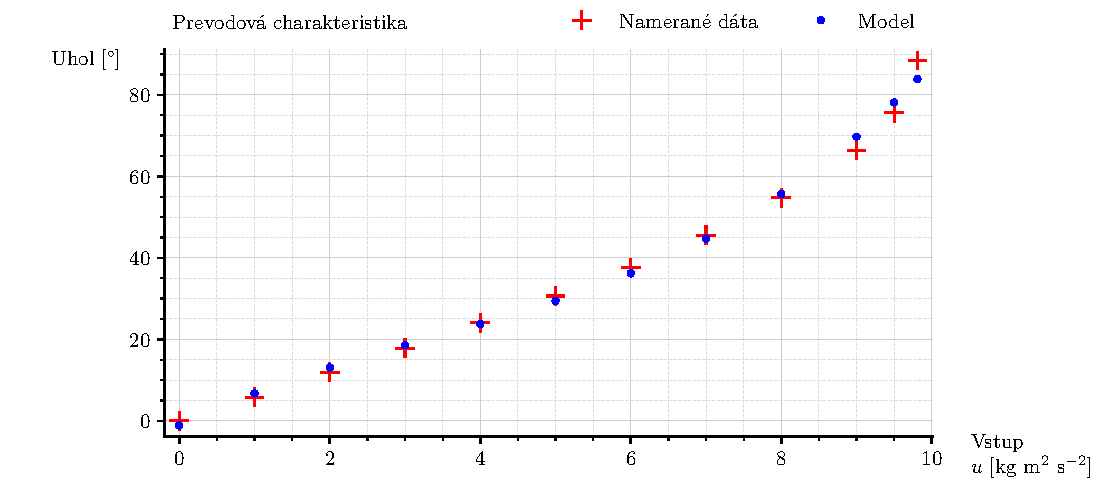
\includegraphics{MRS09_figsc_02_a_2.pdf}
    }

    \vspace{-6pt}

    \figcaption{Prevodová charakteristika}
    \label{Prevodová charakteristika namer vs model}
    }

\end{center}

\subsubsection{Používanie modelu}

Model, samozrejme, umožňuje vypočítať aproximáciu reálneho výstupu pre akúkoľvek hodnotu vstupu - nie len pre hodnoty vstupov, pre ktoré boli merané hodnoty skutočného systému. Vypočítajme výstupy modelu pre tieto vstupné hodnoty (dané vektorom):
\begin{lstlisting}[language=Matlab, numbers=none]
u_ine = [0:0.1:9.81];
\end{lstlisting}
Teda zavoláme funkciu \verb|polyval|.
\begin{lstlisting}[language=Matlab, numbers=none]
y_ine_1 = polyval(polyKoef, u_ine);
\end{lstlisting}
Nakreslime obrázok (viď obr.~\ref{Prevodová charakteristika nuine})
\begin{lstlisting}[language=Matlab, numbers=none]
figure(3);
hold on;
plot(prevodChar(:,1), prevodChar(:,2), '+r')
plot(u_ine, y_ine_1, '.b')
\end{lstlisting}
\begin{center}

    \vbox{%
    \makebox[\textwidth][c]{%
    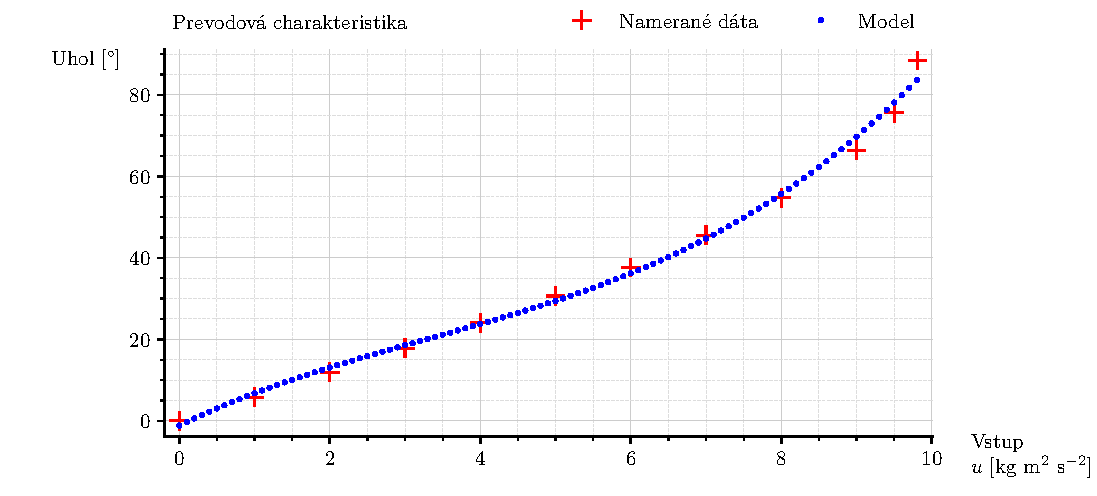
\includegraphics{MRS09_figsc_03_a_3.pdf}
    }

    \vspace{-6pt}

    \figcaption{Prevodová charakteristika}
    \label{Prevodová charakteristika nuine}
    }

\end{center}


















\section{O meraní prechodovej charakteristiky}

Nasledujúci text má za cieľ inšpirovať čitateľa tak, aby získal lepšiu predstavu o~tom ako zrealizovať zmysluplné meranie prechodových charakteristík (aj keď v tomto prípade sa čitateľ bude zaoberať len simuláciami). V tomto prípade totiž nie je úlohou len samotné získanie prechodovej charakteristiky. Potrebný je tiež rozbor problému z hľadiska daného reálneho (simulovaného) systému (ktorého vlastnosti skúmame). Preto je v prvom rade potrebné vysvetlenie pojmov používaných pri opise dynamického systému.

Pripomeňme, že v tomto bode máme dostupnú istú informáciu o predmetnom skúmanom systéme. Je ňou prevodová charakteristika - viď obr.~\ref{Prevodová charakteristika graf}.

Samotná prevodová charakteristika vystihuje tzv. statické vlastnosti systému. Vlastnosti systému v ustálenom stave. Celkom konkrétne je možné z prevodovej charakteristiky získať statické zosilnenie systému.

Prevodová charakteristika na obr.~\ref{Prevodová charakteristika graf} ukazuje, že zosilnenie systému pri nižších hodnotách vstupného signálu je iné ako zosilnenie pri vyšších hodnotách vstupného signálu. Využime skutočnosť, že v tomto prípade máme dostupný model prevodovej charakteristiky (nie je nevyhnutné mať takýto model). Modelom je polynomiálna funkcia, konkrétne:
\begin{equation} \label{modelPolifitVysl2}
    \hat y = 0,1105 u^3  -1,1071 u^2 + 8,8873 u  -1,146
\end{equation}
Použime tento model pre vypočítanie výstupov (odhadov výstupov) systému v týchto hodnotách vstupného signálu:
\begin{lstlisting}[language=Matlab, numbers=none]
u_ine = [0:0.1:9.81];
\end{lstlisting}
Získame obrázok~\ref{Prevodová charakteristika graf2}.
\begin{center}

    \vbox{%
    \makebox[\textwidth][c]{%
    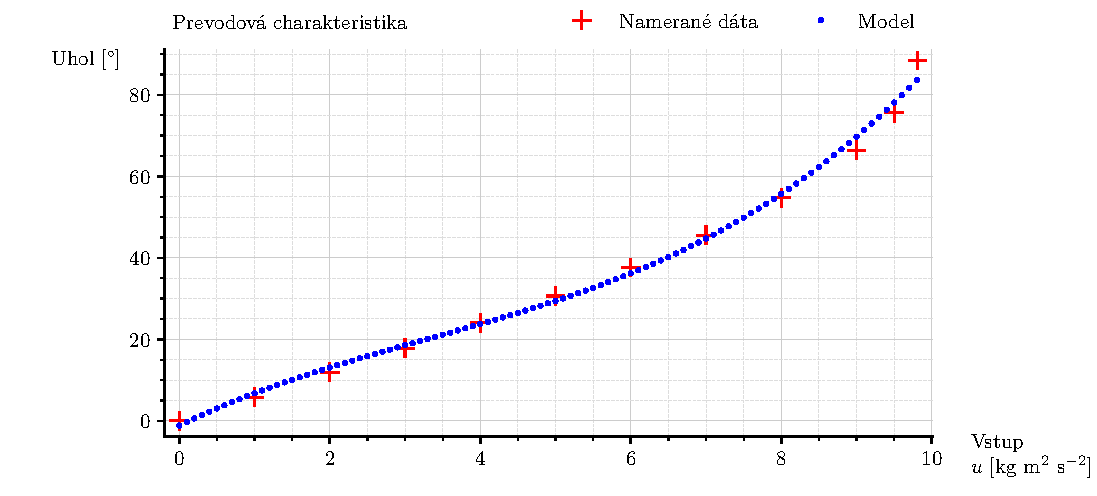
\includegraphics{MRS09_figsc_03_a_666.pdf}
    }

    \vspace{-6pt}

    \figcaption{}
    \label{Prevodová charakteristika graf2}
    }

\end{center}




\subsection{Pracovný bod}

Hlavnou úlohou v tomto texte je získať prechodové charakteristiky predmetného systému (laboratórny systém) v rôznych pracovných bodoch. Pracovné body nech sú zvolené s prihliadnutím na prevodovú charakteristiku systému. V prvom rade, čo je to \emph{pracovný bod}?

Pracovný bod je definovaný ustálenou hodnotou vstupného signálu, ku ktorej (jednoznačne) prislúcha ustálená hodnota výstupného signálu. Dvojica hodnôt, hodnota na vstupe a hodnota na výstupe, tvorí pracovný bod.

Ak je daná ustálená hodnota vstupného signálu, potom je možné pomocou prevodovej charakteristiky nájsť prislúchajúcu ustálenú hodnotu výstupného signálu.

Pojem pracovný bod na seba viaže aj pojem \emph{okolie pracovného bodu}. V okolí pracovného bodu sú vlastnosti systému relatívne rovnaké ako v pracovnom bode. Z~hľadiska statických vlastností systému to znamená, že v okolí pracovného bodu sa sklon prevodovej charakteristiky relatívne nemení. Inými slovami, statické zosilnenie systému sa nemení. Rovnako aj dynamické vlastnosti systému sú v okolí pracovného bodu relatívne nemenné - časové konštanty systému sa nemenia.

V dvoch rôznych pracovných bodoch môže mať reálny systém napríklad rozdielne statické zosilnenie, teda statické vlastnosti. Statické zosilnenie systému v pracovnom bode je možné určiť na základe prevodovej charakteristiky. Je dané sklonom prevodovej charakteristiky v okolí pracovného bodu.

Prípadný rozdiel v statických vlastnostiach v rôznych pracovných bodoch však nehovorí nič o prípadnom rozdiele dynamických vlastnostiach systému. Dynamické vlastnosti je možné vyhodnocovať na základe prechodovej charakteristiky.

\emph{Prechodová charakteristika} je odozva systému na jednotkový skok.

Pod pojmom \emph{jednotkový skok} sa rozumie skoková zmena signálu (vstupného) a veľkosť tejto zmeny je jednotková. Je jednotková zmysle, že akúkoľvek veľkosť skokovej zmeny má zmysel (prípadne) vyjadriť ako násobok jednotkovej skokovej zmeny. Prirodzene sa predpokladá, že jednotková zmena je taká, že nespôsobí, že systém sa dostane mimo okolia pracovného bodu.






\subsection{Voľba pracovných bodov}

Pracovné body nech sú zvolené s prihliadnutím na prevodovú charakteristiku systému. Ako teda prihliadnuť? Ako už bolo uvedené, z prevodovej charakteristiky je zrejmé, že istá vlastnosť systému je iná pri nízkych hodnotách vstupného signálu a iná pri vysokých hodnotách. Tou vlastnosťou je statické zosilnenie. Iné než tzv. statické vlastnosti systému z prevodovej charakteristiky nie je možné vyčítať. Otázkou teda je či sú aj iné vlastnosti systému rozdielne pri rôznych hodnotách vstupného signálu.

Zvoľme preto dva pracovné body - jeden nech reprezentuje nízku hodnotu vstupného signálu a druhý vysokú. Zvolené pracovné body sú uvedené v tabuľke~\ref{Zvolené pracovné body}.
\begin{center}

    \vbox{
    
    \tabcaption{Zvolené pracovné body}
    \label{Zvolené pracovné body}
    
    \begin{tabular}{ccc}
        \toprule
        PB & hodnota & jednotky \\
        \midrule
        1. & $4$ & [kg m$^2$ s$^{-2}$] \\
        2. & $9,5$ & [kg m$^2$ s$^{-2}$] \\
        \bottomrule
    \end{tabular}
    } 
    
\end{center}
Na základe nameraných bodov prevodovej charakteristiky by sme mohli k~zvoleným ustáleným vstupným hodnotám priradiť výstupné hodnoty:

\noindent
\begin{tabular}{@{}l l}
    1.PB: & $y=23,76$ [°] \\
    2.PB: & $y=78,13$ [°]
\end{tabular}


Pracujme však s aproximáciou prevodovej charakteristiky, teda s jej modelom. Model nám umožní získať aj také informácie, ktoré neboli reálne namerané.

Pre $u = 4$ [kg m$^2$ s$^{-2}$] podľa modelu prevodovej charakteristiky prislúcha hodnota ustáleného výstupu:
\begin{equation}
    \hat y_{PB1} = 0,1105\ u_{PB1}^3  -1,1071\ u_{PB1}^2 + 8,8873\ u_{PB1}  -1,146
\end{equation}
kde ak $u_{PB1} = 4$ [kg m$^2$ s$^{-2}$], potom $\hat y_{PB1} = 23,73$ [°]. Podobne pre $u = 9,5$ [kg m$^2$ s$^{-2}$] podľa modelu prevodovej charakteristiky prislúcha hodnota ustáleného výstupu $\hat y_{PB2} = 78,06$ [°]. Znázornime pracovné body - viď obr.~\ref{Prevodová charakteristika graf4}.
\begin{center}

    \vbox{%
    \makebox[\textwidth][c]{%
    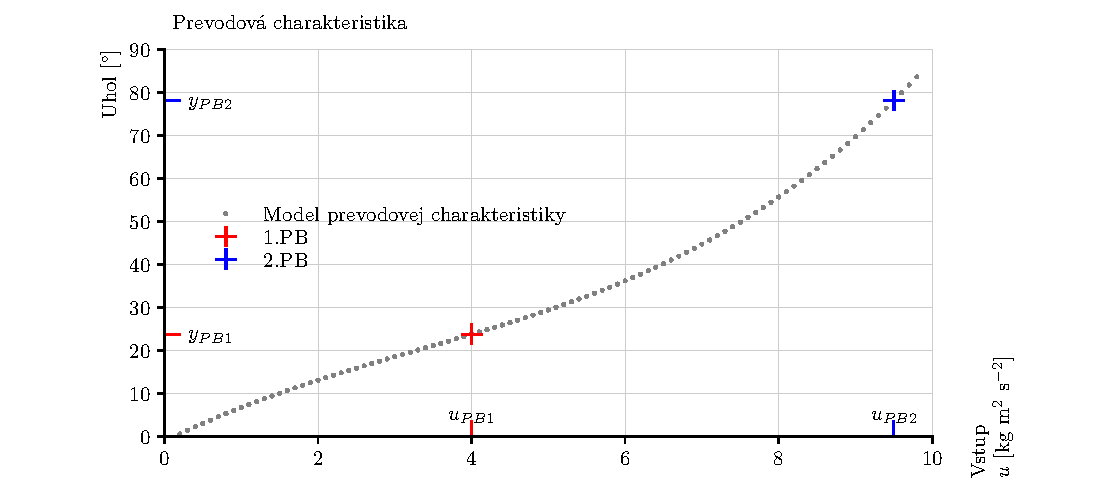
\includegraphics{MRS09_PCH_figsc_04_0.pdf}
    }

    \vspace{-6pt}

    \figcaption{}
    \label{Prevodová charakteristika graf4}
    }

\end{center}
Ďalej je, samozrejme, potrebné vhodne zvoliť okolie pracovného bodu (pre každý pracovný bod). V podstate je potrebné voliť pracovný bod a prislúchajúce okolie pracovného bodu naraz. Len tu sme to pre lepšiu názornosť oddelili.

Pripomeňme, že v okolí pracovného bodu sa očakáva, že vlastnosti systému sú relatívne nemenné. Na základe prevodovej charakteristiky možno posúdiť statické vlastnosti systému. Na základe toho, pre 1. pracovný bod (PB1) zvoľme okolie $u = 4 \pm 0,8$ [kg m$^2$ s$^{-2}$]. Pre PB2 zvoľme $u = 9,5 \pm 0,25$ [kg m$^2$ s$^{-2}$]. Znázornime pracovné body a ich okolia - viď obr.~\ref{Prevodová charakteristika graf5}. Na obrázku~\ref{Prevodová charakteristika graf5} sú tiež vyznačené hranice okolia pracovného bodu, napr. $u_{PB1_l}$ ako dolná hranica okolia pracovného bodu a~$u_{PB1_h}$ ako horná hranica. K tomu zodpovedajúce hodnoty výstupnej veličiny, hodnoty $y_{PB1_l}$ a~$y_{PB1_h}$ sú taktiež vyznačené. Obdobne aj pre druhý pracovný bod.
\begin{center}

    \vbox{%
    \makebox[\textwidth][c]{%
    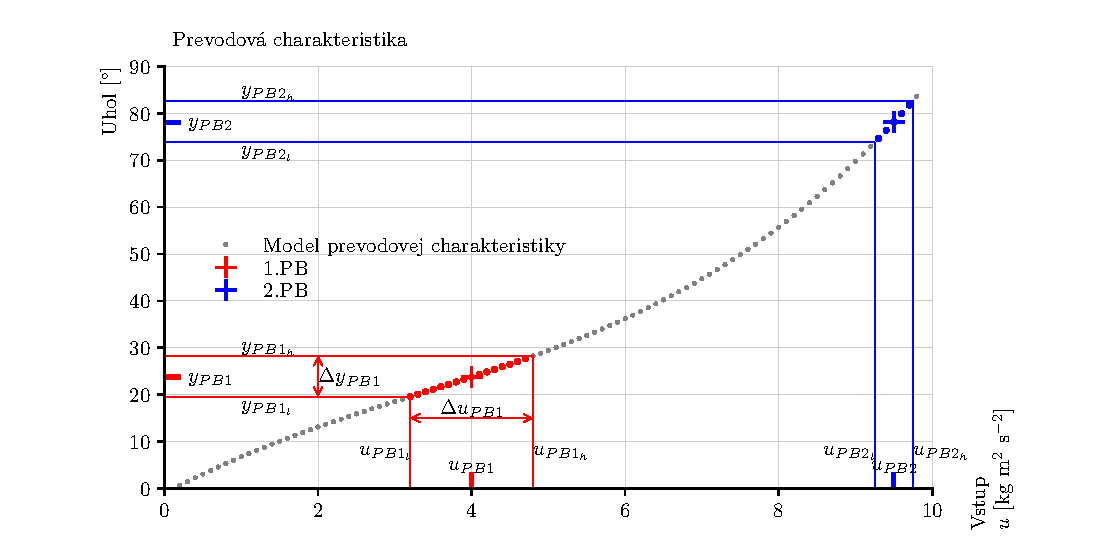
\includegraphics{MRS09_PCH_figsc_05_0.pdf}
    }

    \vspace{-6pt}

    \figcaption{}
    \label{Prevodová charakteristika graf5}
    }

\end{center}
Ďalej je v tomto prípade potrebné uvážiť veľkosť skokovej zmeny, ktorú budeme používať ako jednotkovú. Vzhľadom na okolnosti nie je dôvod, aby jednotkovou veľkosťou nebola hodnota definujúca okolie pracovného bodu. Spĺňa sa tak požiadavka, že jednotkový skok nespôsobí, že systém sa dostane mimo okolia pracovného bodu (bude na hrane, ale nie mimo). Preto pre PB1 nech je jednotková veľkosť skokovej zmeny rovná hodnote $u_{s1} = 0,8$ [kg m$^2$ s$^{-2}$] a pre PB2 nech je jednotková veľkosť skoku rovná hodnote $u_{s2} = 0,25$ [kg m$^2$ s$^{-2}$].





\subsection{Zrealizovanie merania prechodovej charakteristiky}

Aby bolo možné vykonať jednotkový skok (skokovú zmenu vstupného signálu systému s~jednotkovou veľkosťou) v okolí pracovného bodu najskôr je potrebné dostať systém do pracovného bodu. Ak bude hodnota vstupného signálu $u_{PB}$, a necháme ju tak nejaký čas, potom očakávame, na základe prevodovej charakteristiky, že výstup systému sa ustáli na hodnote $y_{PB}$. Systém bude v pracovnom bode. Potom je možné skokovo zvýšiť hodnotu vstupného signálu o hodnotu $u_{s}$. Tým sa zrealizuje jednotkový skok v~okolí pracovného bodu. Simulácia uvedeného je na obr.~\ref{graf6}.
\begin{center}

    \vbox{%
    \makebox[\textwidth][c]{%
    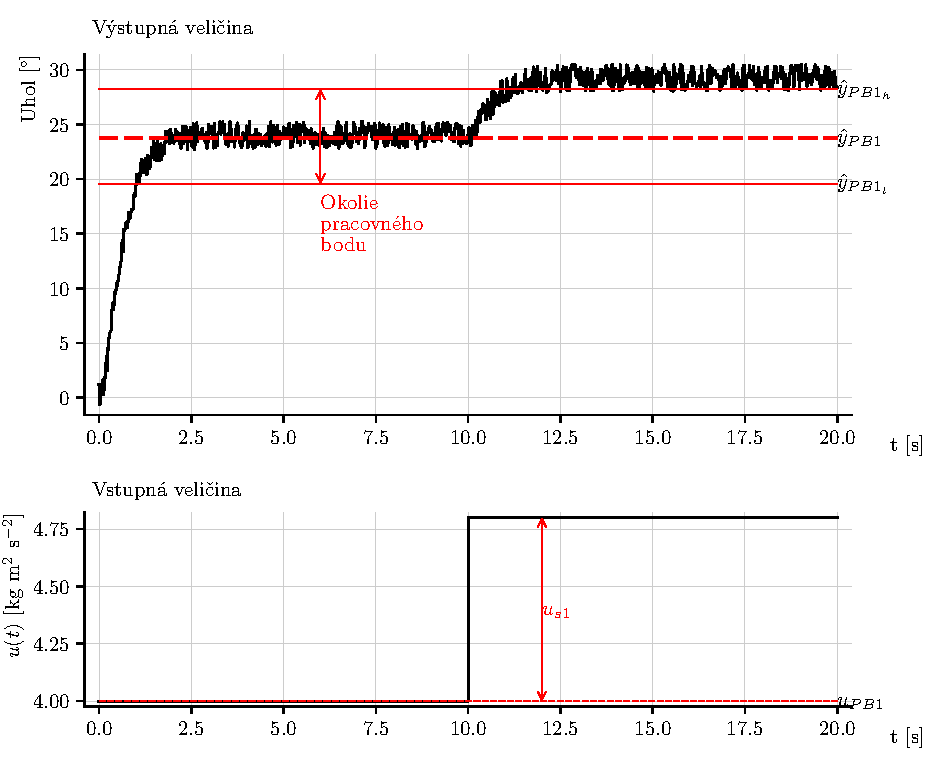
\includegraphics{MRS09_PCH_figsc_06_0.pdf}
    }

    \vspace{-6pt}

    \figcaption{}
    \label{graf6}
    }

\end{center}
Veľkosť skokovej zmeny vstupného signálu je na obrázku~\ref{graf6} označená ako $u_{s1}$. V~tomto prípade, vzhľadom na zvolené okolie pracovného bodu, je $u_{s1} = 0,8$.

Jednotkový skok nastal v čase $t=10$ [s]. Pred týmto časom sa systém dostával do pracovného bodu. Od času $t=10$ [s] až pokým sa výstupná veličina systému opäť neustálila prebieha prechodový dej, to je prechodová charakteristika (keďže na vstupe bol jednotkový skok).






\subsection{Spracovanie nameraného}


Pred jednotkovým skokom sme očakávali, že výstupná veličina sa ustáli na hodnote $y_{PB}$. Podľa modelu prevodovej charakteristiky to pre tento pracovný bod je hodnota $\hat y_{PB1} = 23,73$ [°]

Priemerná hodnota výstupnej veličiny počas doby 5 sekúnd pred jednotkovým skokom je $24,04$ [°]. Odchýlka priemernej hodnoty, okolo ktorej sa systém ustálil v~pracovnom bode, od očakávanej hodnoty podľa modelu prevodovej charakteristiky je približne 1 \%. To je samozrejme prijateľná odchýlka. Ďalej teda môžeme považovať hodnotu $\hat y_{PB1}$ podľa modelu prevodovej charakteristiky za hodnotu, na ktorej bola ustálená výstupná veličina pred skokovou zmenou vstupného signálu.

Po ukončení prechodového deja sa podľa modelu prevodovej charakteristiky očakáva, že výstupná veličina sa ustáli na hodnote $\hat y_{PB1_h} = 28,19$ [°]

Už z obr.~\ref{graf6} je zrejmé, že v skutočnosti sa výstupná veličina ustáli na o niečo vyššej hodnote. Presnejšie, ak uvažujeme časový úsek po jednotkovom skoku, na ktorom je už výstupná veličina ustálená, nech je to úsek 2,5 až 5 sekúnd po jednotkovom skoku, tak na tomto úseku je priemerná hodnota výstupnej veličiny $29,2$ [°].

Ak pri hodnote $y_{PB1}$ bol rozdiel medzi očakávaným (podľa modelu prevodovej charakteristiky) a nameraným priam zanedbateľný, pri hodnote $y_{PB1_h}$ to už nie je také jednoznačné. Nie je jednoznačné, že rozdiel je zanedbateľný. Tento problém však súvisí s meraním prevodovej charakteristiky a následnou voľbou modelu prevodovej charakteristiky, ktorý sme sa tu rozhodli používať pri odhadovaní očakávaných hodnôt $y_{PB1}$ a $y_{PB1_h}$. Ak sme sa raz rozhodli používať daný model prevodovej charakteristiky, potom s prípadnými odchýlkami, ktoré zjavne nie sú omyly, je potrebné počítať.

Týmto sme chceli povedať, že napriek tomu, že čo sa očakávaných hodnôt týka, po jednotkovom skoku výstupná veličina opustila očakávané okolie pracovného bodu. Avšak je to len očakávané, odhadované okolie (na základe modelu prevodovej charakteristiky). Odchýlky od „reálnych“ hodnôt sú prijateľné a teda môžeme pokračovať bez nutnosti prehodnotiť voľbu okolia pracovného bodu.




\subsubsection{„Vystrihnutie“ prechodovej charakteristiky}

Vyberme z dát na obr.~\ref{graf6} len tú časť, ktorá zodpovedá prechodovej charakteristike, teda dáta od času 10 až po ustálenie (nech je to čas 15). Výsledkom je obr.~\ref{graf7}.
\begin{center}

    \vbox{%
    \makebox[\textwidth][c]{%
    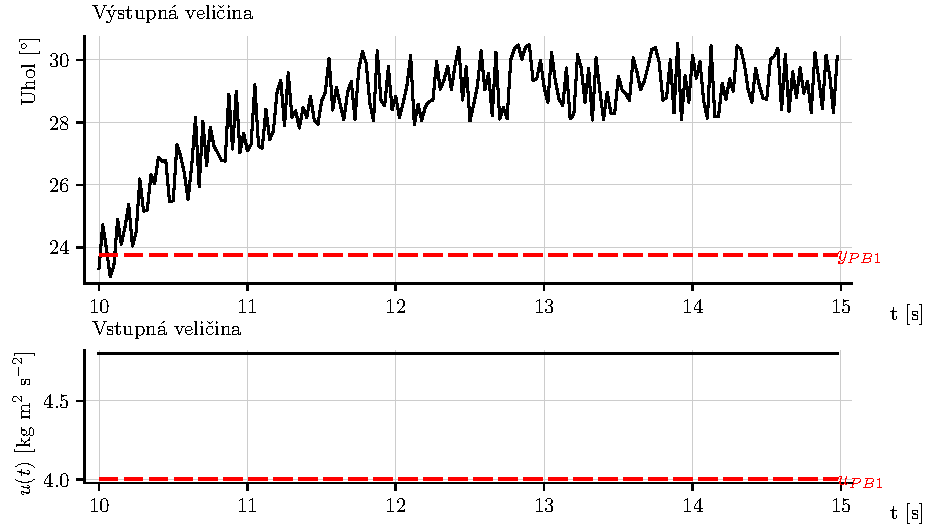
\includegraphics{MRS09_PCH_figsc_07_0.pdf}
    }

    \vspace{-6pt}

    \figcaption{}
    \label{graf7}
    }

\end{center}



\subsubsection{„Posunutie“ prechodovej charakteristiky}

Pre potreby ďalšej práce s prechodovou charakteristikou je zvyčajne výhodné posunúť namerané dáta tak aby začiatok prechodovej charakteristiky bol v bode (0,0), to znamená, že PCH začína v  čase 0 a hodnota výstupnej veličiny v začiatku je tiež nula (aspoň filozoficky).

Konkrétne: od získaného priebehu výstupnej veličiny je potrebné odčítať hodnotu $y_{PB}$, pretože tak sa začiatok posunie v smere osi y do nuly (filozoficky... teraz nám to asi bude kaziť šum). Rovnako priebeh vstupnej veličiny je potrebné posunúť v~smere osi o hodnotu $u_{PB}$. Samozrejme, od časového vektora je potrebné odčítať čas, v~ktorom nastal jednotkový skok. Výsledok je na obr.~\ref{graf8}.
\begin{center}

    \vbox{%
    \makebox[\textwidth][c]{%
    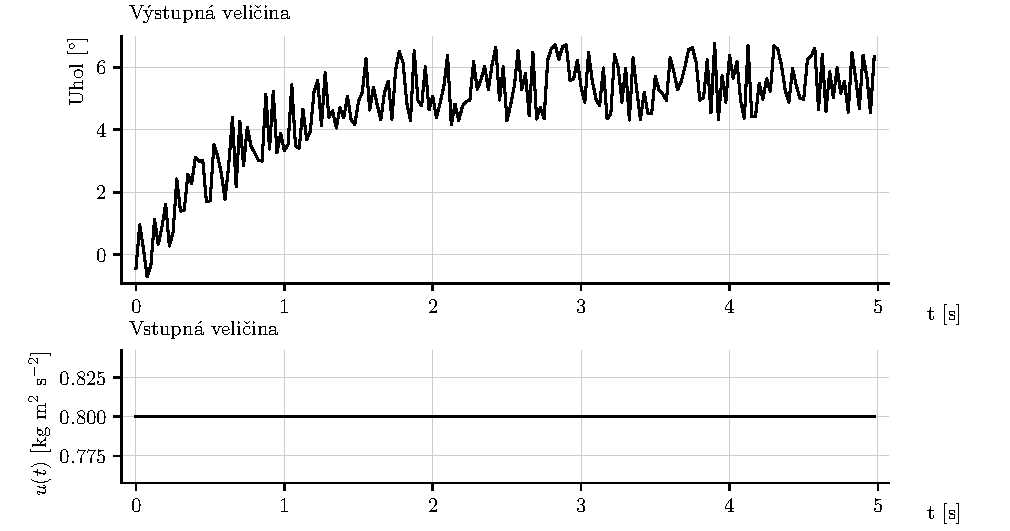
\includegraphics{MRS09_PCH_figsc_08_0.pdf}
    }

    \vspace{-6pt}

    \figcaption{}
    \label{graf8}
    }

\end{center}




\subsection{Poznámky k odčítavaniu hodnôt z grafu prechodovej charakteristiky}



\subsubsection{Nameraná prechodová charakteristika}

Z predchádzajúceho je dostupná nameraná a spracovaná prechodová charakteristika (PCH) predmetného systému. Ide o prechodovú charakteristiku v prvom pracovnom bode. Je zobrazená na obr.~\ref{graf8}.

Ďalej sú dostupné informácie o pracovnom bode, v ktorom bola PCH meraná. Hodnota vstupného signálu v pracovnom bode je $u = 4$ [kg m$^2$ s$^{-2}$] a uvažuje sa okolie pracovného bodu $u = 4 \pm 0,8$ [kg m$^2$ s$^{-2}$].

Je dostupný podel prevodovej charakteristiky a teda je možné odhadnúť hodnotu výstupnej veličiny v pracovnom bode, teda
\begin{equation}
    \hat y_{PB1} = 0,1105\ u_{PB1}^3  -1,1071\ u_{PB1}^2 + 8,8873\ u_{PB1}  -1,146
\end{equation}
kde $u_{PB1} = 4$ [kg m$^2$ s$^{-2}$] a teda $\hat y_{PB1} = 23,73$ [°]. Rovnako je možné vypočítať hodnotu výstupného signálu pre, nazvime to, hornú hranicu okolia pracovného bodu, to znamená pre hodnotu na vstupe $u_{PB1_h} = 4 + 0,8$ [kg m$^2$ s$^{-2}$]. Tejto zodpovedá hodnota $\hat y_{PB1_h} = 28.19$ [°].

Keďže prechodová charakteristika na obr.~\ref{graf8} je posunutá do nuly, teda od skutočných hodnôt sú odčítané hodnoty v pracovnom bode, tak urobme túto úpravu aj pre práve vypočítané hodnoty, teda
\begin{align}
    \Delta u_{PB1} &= u_{PB1_h} - u_{PB1} = 0,8 \\
    \Delta \hat y_{PB1} &= \hat y_{PB1_h} -  \hat y_{PB1} = 4,52
\end{align}



\subsubsection{Statické zosilnenie $K$}

Zistime statické zosilnenie systému v okolí uvažovaného pracovného bodu. Potrebujeme hodnotu, na ktorej sa ustálila výstupná veličina po prechodovom deji. Z grafu PCH uvažujme, že výstupná veličina je už ustálená po čase $t=3$ [s] (dajme tomu teraz takto). Priemerná hodnota výstupnej veličiny po tomto čase je $\Delta y = 5.52$ [°].

Teda, po uskutočnení jednotkového skoku v okolí pracovného bodu sa výstupná veličina zmenila o $\Delta y$ [°]. Zmena na vstupe $\Delta u$ bola, samozrejme, práve jednotková (pretože jednotkový skok). V tomto prípade má jednotkový skok veľkosť okolia pracovného bodu  $\Delta u = 0,8$ [kg m$^2$ s$^{-2}$].

Statické zosilnenie systému, na základe prechodovej charakteristiky, označme $K$, je $K = \frac{\Delta y}{\Delta u}$, číselne
\begin{equation}
     K = 6,9 \text{[°/(kg m$^2$ s$^{-2}$)]}
\end{equation}
Uvedené možno znázorniť aj do grafu - viď obr.~\ref{graf20}
\begin{center}

    \vbox{%
    \makebox[\textwidth][c]{%
    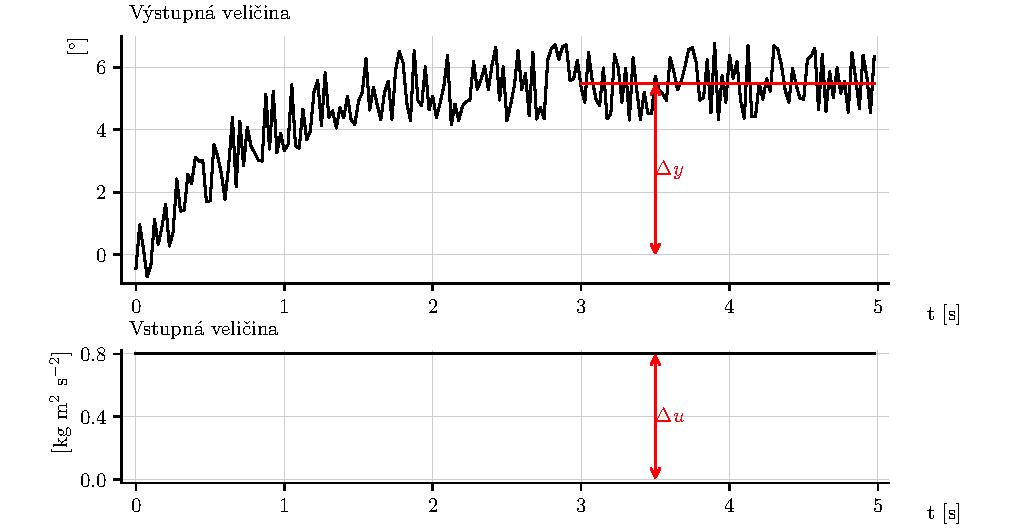
\includegraphics{MRS09_PCH_figsc_10_02_0.pdf}
    }

    \vspace{-6pt}

    \figcaption{}
    \label{graf20}
    }

\end{center}

Statické zosilnenie systému je, samozrejme, možné zistiť aj pomocou prevodovej charakteristiky. V skutočnosti, všetko potrebné už máme k dispozícii.

Mimochodom, ak by sme neboli leniví, tak nájdeme dotyčnicu v pracovnom bode, a jej smernica (sklon) by mala byť statické zosilnenie. To by bol formálne korektný postup.

My však leniví sme, preto: hľadáme sklon prevodovej charakteristiky v okolí pracovného bodu. Z praktického hľadiska, nech je sklon daný pracovným bodom a bodom ohraničujúcim okolie pracovného bodu zhora. Formálne $\text{sklon} = \frac{\Delta y}{\Delta u}$ kde $\Delta y = \hat y_{PB_h} - \hat y_{PB}$ a~$\Delta u = u_{PB_h} - u_{PB}$. To je, samozrejme, to isté ako vyplynulo z~využitia prechodovej charakteristiky vyššie. Tu však číselné hodnoty nie sú odčítané z~prechodovej charakteristiky ale z~modelu prevodovej charakteristiky. Konkrétne čísla:
\begin{equation}
    \text{sklon} = \frac{\hat y_{PB_h} - \hat y_{PB}}{u_{PB_h} - u_{PB}} = \frac{4,52}{0,8} = 5.65
\end{equation}
Odchýlka od statického zosilnenia určeného z prechodovej charakteristiky je $-1,25$ [°], t.j. $18,10$ [\%] (tá je samozrejme daná aj tým, že používame model prevodovej charakteristiky, keďže konkrétne potrebné hodnoty v rámci nameranej prevodovej charakteristiky nie sú dostupné).




\subsubsection[Časová konštanta $T$ pre lineárny dynamický systém 1. rádu]{Časová konštanta $T$ pre lineárny dynamický systém 1. rádu}


Ďalej je možné nájsť model, ktorý má vystihovať dynamiku (dynamické vlastnosti) reálneho systému. Modelom nech je lineárny dynamický systém.

Kvalifikovaný odhad založený na grafickom znázornení predmetnej prechodovej charakteristiky vedie k možnosti, že modelom systému môže byť dynamický systém 1. rádu. Tento je možné zapísať v tvare prenosovej funkcie
\begin{equation}
    G(s) = \frac{y(s)}{u(s)} = \frac{K}{Ts+1}
\end{equation}
kde $K$ je možné interpretovať ako statické zosilnenie systému a $T$ je časová konštanta.

Časovú konštantu je možné nájsť na základe prechodovej charakteristiky. Je to čas od začiatku prechodovej charakteristiky (od času jednotkového skoku), v ktorom výstupná veličina dosiahla približne 63 \% zo svojej ustálenej hodnoty.

Prečo práve 63 \%? Odpoveď sa ponecháva na čitateľa.

100 \% z ustálenej hodnoty na nasledujúcom obrázku~\ref{graf30} je samozrejme hodnota $\Delta y$. Potom 63 \% je hodnota $\Delta y_{63} =  3,48$ [°]
\begin{center}

    \vbox{%
    \makebox[\textwidth][c]{%
    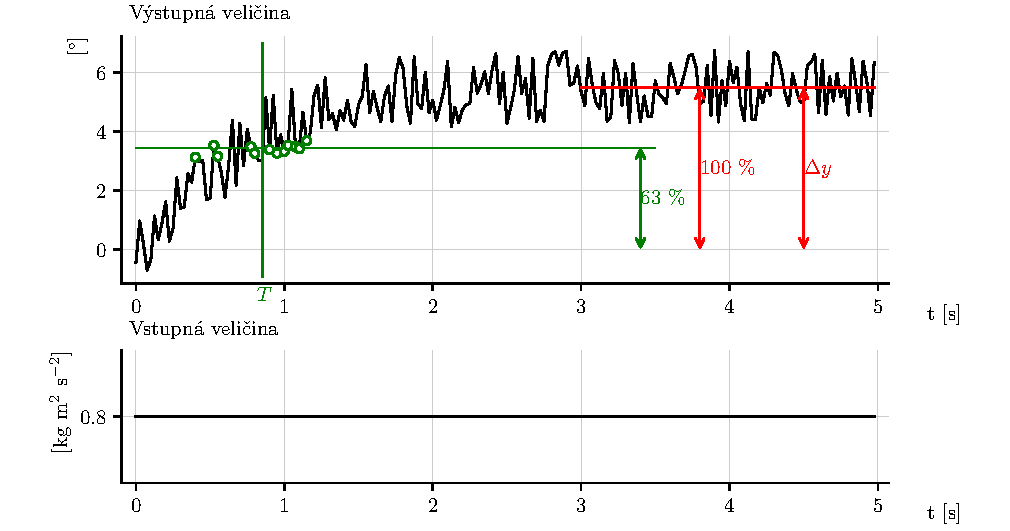
\includegraphics{MRS09_PCH_figsc_10_03_0.pdf}
    }

    \vspace{-6pt}

    \figcaption{}
    \label{graf30}
    }

\end{center}
Hodnotu $T$ teraz možno hľadať „od oka“, doslova pomocou grafu PCH, prípadne „od oka“, ale trošku inak - napr: Nájdime hodnoty výstupnej veličiny, ktoré sú v~pásme (volajme ho „od oka“) $\pm ? \%$ v okolí hodnoty $\Delta y_{63}$. Presnejšie, nájdime časy tých vzoriek, ktoré sú v~tom pásme. Nájdené body v~pásme „od oka“ okolo hodnoty $\Delta y_{63}$ sú na obr.~\ref{graf30} vyznačené ako malé zelené kružnice. Priemer z nájdených časov je
\begin{equation}
    T =  0,81 \text{[s]}
\end{equation}
A táto hodnota môže byť celkom dobre „od oka“ odčítaná časová konštanta. Všetko uvedené je nakreslené na obr.~\ref{graf30}.




\subsubsection{Verifikácia identifikovaného dynamického modelu}


V predchádzajúcom boli na základe prechodovej charakteristiky určené parametre lineárneho dynamického systému, ktorý má byť modelom skutočného systému. Tento model je možné vyjadriť v tvare prenosovej funkcie
\begin{equation}
    \frac{y(s)}{u(s)} = \frac{K}{Ts+1}
\end{equation}



Pre verifikáciu modelu je možné využiť grafické porovnanie prechodovej charakteristiky modelu a skutočnej prechodovej charakteristiky. Pre získanie PCH modelu využime numerickú simuláciu. Daná prenosová funkcia zodpovedá diferenciálnej rovnici v tvare
\begin{align}
    T \dot y(t) + y(t) &= K u(t) \\
    T \dot y(t) &= - y(t) + K u(t) \\
    \dot y(t) &= - \frac{1}{T} y(t) + \frac{K}{T} u(t)
\end{align}
Vstupný signál zvoľme rovnaký ako je veľkosť $\Delta u$. Tak zabezpečíme zodpovedajúcu veľkosť jednotkového skoku, ktorý je použitý v numerickej simulácii pre získanie PCH.

Do spoločného obrázka nakreslime nameranú PCH a PCH modelu systému - viď obr.~\ref{graf40}
\begin{center}

    \vbox{%
    \makebox[\textwidth][c]{%
    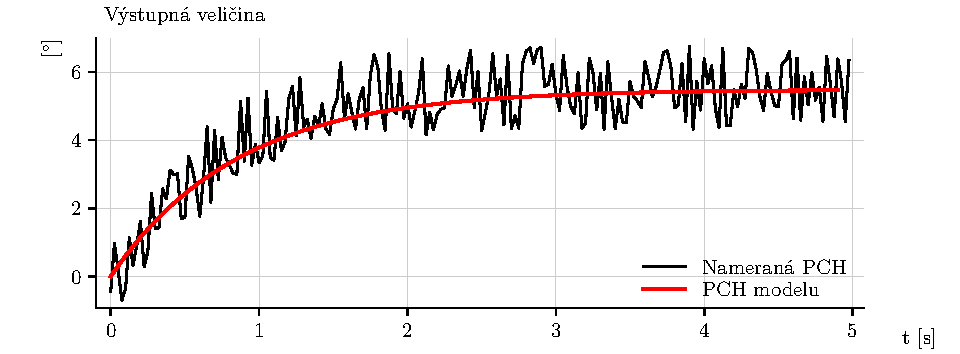
\includegraphics{MRS09_PCH_figsc_10_04_0.pdf}
    }

    \vspace{-6pt}

    \figcaption{}
    \label{graf40}
    }

\end{center}
Týmto (aspoň pre naše potreby) možno model považovať za verifikovaný - znamená to, že daný model je schopný vystihnúť vlastnosti skutočného systému a že je možné na základe dostupných informácií (prechodová charakteristika) nájsť parametre modelu.














\section{Doplnkový text: O stabilite dynamického systému}


Pripomeňme matematický model kyvadla, ktorým sme sa zaoberali v predchádzajúcich témach.
Pohybová rovnica opisujúca dynamiku rotačného pohybu kyvadla je v tvare
\begin{align} \label{PohRovKyvadla} %\label{PohRovKyvadlab}
		&ml^2 \ddot{\varphi} = -\beta \dot{\varphi} - mgl\sin{\varphi} + u
\end{align}
pričom ide o kyvadlo, ktorého kmity sú tlmené viskóznym trením s~koeficientom $\beta$ [kg~m$^2$~s$^{-1}$], hmotný bod s~hmotnosťou $m$ [kg] pripevnený na ramene so zanedbateľnou hmotnosťou a~dĺžkou $l$ [m] kmitá okolo osi otáčania a uhol od zvislice je označený $\varphi$ [rad]. $g$~[m~s$^{-2}$] je gravitačné zrýchlenie. 
% Číselné hodnoty parametrov kyvadla sú uvedené v tabuľke~\ref{Parametre kyvadla}.

Ďalej sme uvažovali, že stavom kyvadla sú dve veličiny: uhol natočenia ramena kyvadla $\varphi$ a~uhlová rýchlosť ramena kyvadla $\dot\varphi$. Stavový vektor má preto dva prvky $x^{\mathsf{T}} = \begin{bmatrix} x_1 & x_2	\end{bmatrix}$, kde $x_1 = \varphi$ a~$x_2 = \dot\varphi$. Model kyvadla v stavovom priestore je v tvare
\begin{subequations}
	\begin{align}
		\begin{bmatrix}
			\dot{x}_1 \\ \dot{x}_2
		\end{bmatrix}
		&=
		\begin{bmatrix}
			x_2 \\ - \frac{\beta}{ml^2} x_2 - \frac{g}{l} \sin(x_1)
		\end{bmatrix}
		+
		\begin{bmatrix}
			0 \\ \frac{1}{ml^2}
		\end{bmatrix}
		u \\
		\varphi &= x_1
	\end{align}
\end{subequations}
Toto je nelineárny časovo-invariantný systém druhého rádu.

V tejto časti budeme uvažovať predmetný dynamický systém, avšak bez vstupu, inými slovami externý moment sily je nulový, $u(t) = 0$. Potom
\begin{subequations}
	\begin{align} \label{fajnVektRov}
		\begin{bmatrix}
			\dot{x}_1 \\ \dot{x}_2
		\end{bmatrix}
		&=
		\begin{bmatrix}
			x_2 \\ - \frac{\beta}{ml^2} x_2 - \frac{g}{l} \sin(x_1)
		\end{bmatrix}
 \\
		\varphi &= x_1
	\end{align}
\end{subequations}





\subsection{Vektorové pole, fázový portrét, ekvilibrium}

Kvalitatívne správanie sa nelineárneho dynamického systému je dôležité pre porozumenie kľúčovým konceptom Lyapunovovej teórie stability systémov. Pre analýzu je dôležitá istá trieda systémov nazývaná planárne dynamické systémy. Tieto systémy majú dve stavové veličiny $x \in \mathbb{R}^2$, čo umožňuje znázorniť stavový priestor v rovine so súradnicovým systémom $(x_1, x_2)$. Navyše výsledky kvalitatívnej analýzy platia vo všeobecnosti a~môžu byť použité aj pri systémoch vyššieho rádu. Preto sú tieto systémy dôležité z hľadiska analýzy. Do tejto triedy systémov patrí aj model kyvadla.

Výhodným spôsobom ako porozumieť správaniu dynamického systému so stavom $x \in \mathbb{R}^2$ je nakresliť \emph{fázový portrét systému}. Začneme zavedením konceptu \emph{vektorového poľa}. Pre systém obyčajných diferenciálnych rovníc zapísaných kompaktne vo vektorovej rovnici (ako rovnica \eqref{fajnVektRov}) v tvare
\begin{align}
	\dot{x} = F(x)
\end{align}
pravá strana rovnice definuje v každom $x \in \mathbb{R}^n$ rýchlosť $F(x) \in \mathbb{R}^n$. Táto rýchlosť hovorí o tom ako sa $x$ mení a~môže byť reprezentovaná vektorom.

Pri planárnom dynamickom systéme, každý stav zodpovedá bodu v rovine a $F(x)$ je vektor rýchlosti reprezentujúci veľkosť a smer zmeny (rýchlosti) daného stavu. Tieto vektory môžme vykresliť na mriežke bodov v rovine a získať tak vizuálny obraz dynamiky systému, tak ako na Obr.~\ref{Vektorové pole znázorňujúce dynamiku kyvadla}. 
% Pre vykreslenie tohto vektorového poľa boli použité parametre kyvadla uvedené v~Tabuľke~\ref{Parametre kyvadla} a tieto parametre budú používané aj v~ďalšom.
\begin{center}

    \vbox{%
    \makebox[\textwidth][c]{%
    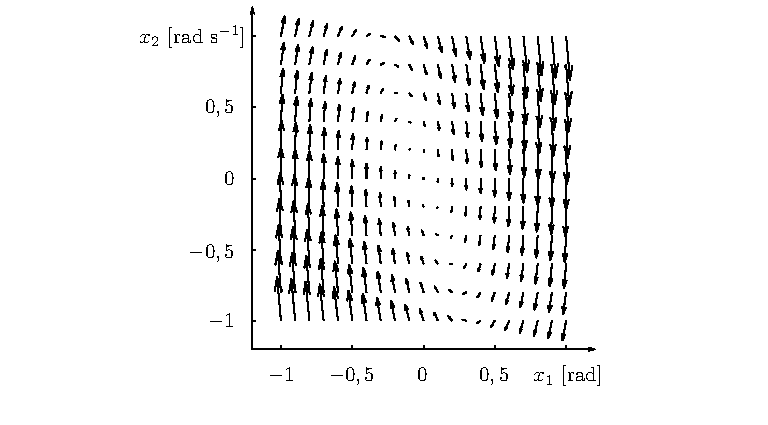
\includegraphics{Obr_KyvydloVektField.pdf}
    }

    \vspace{-6pt}

    \figcaption{Vektorové pole znázorňujúce dynamiku kyvadla (obrázok vytvorený v~MATLABe, viď text)}
    \label{Vektorové pole znázorňujúce dynamiku kyvadla}
    }

\end{center}




\paragraph{Vektorové pole}


Vektorové pole na obr.~\ref{Vektorové pole znázorňujúce dynamiku kyvadla} bolo vygenerované v~Matlabe použitím nasledujúceho kódu:
\begin{lstlisting}[language=Matlab, title=Kód pre vygenerovanie obr.~\ref{Vektorové pole znázorňujúce dynamiku kyvadla}]
m = 1; %kg
l = 1; %m
g = 9.81; %m/s^2
beta = 2*0.5*sqrt(g/l); %kgm^2/s
[x1, x2] = meshgrid(-1:.1:1, -1:.2:1);
x1dot = x2;
x2dot = -(beta/m*l^2).*x2 - (g/l).*sin(x1);
quiver(x1,x2,x1dot,x2dot,1.5);
axis([-1.2 1.2 -1.2 1.2])
axis equal
\end{lstlisting}

Body, v ktorých je vektor rýchlosti nulový sú obzvlášť zaujímavé, pretože definujú stacionárne body systému: ak je autonómny systém v~takom stave na začiatku, ostane v tom stave po celý čas.


\paragraph{Fázový portrét}

Fázový portrét (nazývaný aj Fázový diagram) pozostáva z \uv{prúdnic} nakreslených podľa vektorového poľa. Inými slovami, pre istú množinu začiatočných stavov vykreslíme riešenia diferenciálnej rovnice v~rovine a~smer pohybu v stavovom priestore vyznačíme šípkou. To zodpovedá sledovaniu \uv{šípky vektorového poľa} v~každom bode stavového priestoru a nakresleniu výslednej trajektórie. Po vykreslení niekoľkých trajektórii pre rôzne začiatočné stavy získame fázový portrét ako na Obr.~\ref{Fázový portrét kyvadla}.
\begin{center}

    \vbox{%
    \makebox[\textwidth][c]{%
    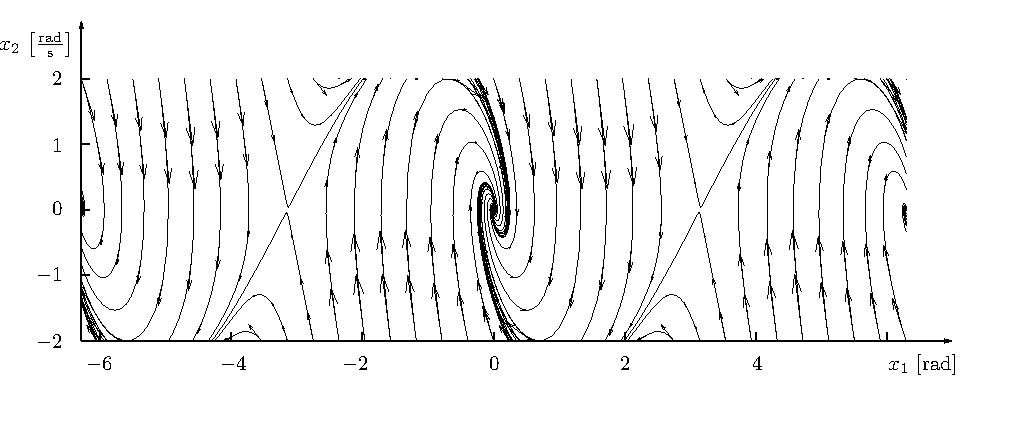
\includegraphics{Obr_KyvadloFazPortret.pdf}
    }

    \vspace{-6pt}

    \figcaption{Fázový portrét kyvadla (obrázok vytvorený v Matlabe, viď text pre zdrojový kód)}
    \label{Fázový portrét kyvadla}
    }

\end{center}
Zdrojový kód pre MATLAB pre získanie tohto obrázku je nasledovný:
\begin{lstlisting}[language=Matlab, title=Kód pre vygenerovanie obr.~\ref{Fázový portrét kyvadla}]
global m l g beta
m = 1; %kg
l = 1; %m
g = 9.81; %m/s^2
beta = 2*0.5*sqrt(g/l); %kgm^2/s

for uhlovarychlost = -2:4:2
  for uhol = -360:22.5:360
    [t,x]=ode45(@PravaStr,[0 5],[uhol*pi/180 uhlovarychlost]);
    hold on
    stav = x;
    x = x(1:5:end-70,:);
    x1dot = x(:,2);
    x2dot=-(beta/m*l^2)*x(:,2)-(g/l)*sin(x(:,1));
    quiver(x(:,1),x(:,2),x1dot,x2dot,0.5,'k')
    plot(stav(:,1),stav(:,2),'k');
    hold off
  end
end

axis equal
axis([-2*pi 2*pi -2 2])
\end{lstlisting}
kde funkcia \verb|PravaStr| je
\begin{lstlisting}[language=Matlab]
function dotx = PravaStr(t,x)
  global m l g beta
  dotx(1)=x(2);
  dotx(2)=-(beta/m*l^2)*x(2)-(g/l)*sin(x(1));
  dotx=dotx';
end
\end{lstlisting}


Fázový portrét je nástroj, ktorý umožňuje posudzovať celkovú dynamiku systému pomocou vykreslenia niekoľkých riešení v stavovom priestore (rovine) systému. Napríklad je možné vidieť, či sa všetky trajektórie s narastajúcim časom približujú k jednému bodu alebo či ide o komplikovanejšie správanie systému. Fázový portrét však nehovorí o veľkosti rýchlosti zmeny stavu (avšak toto môže byť odvodené z dĺžky vektorov vo vektorovom poli systému).




\paragraph{Ekvilibrium}

Ekvilibrium dynamického systému je bod v stavovom priestore, ktorý reprezentuje rovnovážne podmienky pre dynamiku systému. Ide o stacionárny bod, v ktorom je vektor rýchlosti trajektórie systému nulový, ako už bolo uvedené.

Hovoríme, že stav $x_e$ je ekvilibrium dynamického systému
\begin{equation*}
	\dot{x} = F(x)
\end{equation*}
ak $F(x_e) = 0$. Ak má autonómny systém začiatočnú podmienku $x(0) = x_e$, potom ostane v tomto stave a~riešenie má tvar $x(t) = x_e$ po celý čas $t>0$, kde sme uvažovali začiatočný čas $t_0 = 0$.

Stacionárne body (ekvilibriá) patria medzi najdôležitejšiu vlastnosť dynamického systému, pretože definujú stavy s nemennými pracovnými podmienkami systému. Systém môže mať nula, jeden alebo viac stacionárnych bodov.

Stacionárne body uvažovaného kyvadla sú
\begin{equation}
	x_e = \begin{bmatrix} \pm n \pi \\ 0 \end{bmatrix}
\end{equation}
kde $n = 0,1,2,\ldots$. Pre párne $n$ sú to stavy keď kyvadlo visí smerom dole a pre nepárne $n$ je kyvadlo v inverznej polohe. Fázový portrét na Obr.~\ref{Fázový portrét kyvadla} je nakreslený pre $-2\pi \leq x_1 \leq 2\pi$, teda na obrázku je päť stacionárnych bodov.



\subsection{Stabilita dynamického systému vo všeobecnosti}


Pripomeňme, že sa zaoberáme autonómnym systémom (homogénnou diferenciálnou rovnicou) v tvare
\begin{equation} \label{vusetrovanySystem}
	\dot{x} = F(x)
\end{equation}
a tiež pripomeňme, čo rozumieme pod pojmom riešenie systému, alebo skrátene riešenie. Hovoríme, že $x(t)$ je \emph{riešenie} diferenciálnej rovnice \eqref{vusetrovanySystem} na časovom intervale od $t_0 \in \mathbb{R}$ do $t_f \in \mathbb{R}$ ak
\begin{equation}
	\frac{\text{d}x(t)}{\text{d}t} = F \big( x(t)  \big) \qquad \text{pre} \; t_0 < t < t_f
\end{equation}
Daná diferenciálna rovnica môže mať mnoho riešení, najčastejšie nás však zaujíma úloha so zadaným začiatočným stavom, inými slovami so zadanými začiatočnými podmienkami, kedy $x(t)$ je predpísané v začiatočnom čase $t_0$ a úlohou je nájsť riešenie vyhovoujúce pre celý budúci čas $t>t_0$. Vtedy $x(t)$ je riešenie diferenciálnej rovnice \eqref{vusetrovanySystem} so začiatočným stavom $x_0 \in \mathbb{R}^n$ v čase $t_0$ ak
\begin{equation}
	x(t_0) = x_0 \quad \text{a} \quad \frac{\text{d}x(t)}{\text{d}t} = F \big( x(t)  \big) \quad \text{pre} \; t_0 < t < t_f
\end{equation}
Najčastejšie sa stretávame s diferenciálnymi rovnicami, pre ktoré existuje jedinečné riešenie, navyše pre celý čas $t>t_0$ čo znamená že $t_f = \infty$. Častým je tiež, že funkcia $F$ je nezávislá od času, preto môžme uvažovať $t_0 = 0$.


\emph{Stabilita riešenia} určuje či iné riešenia v~blízkosti skúmaného riešenia ostávajú v~jeho blízkosti, približujú sa k~nemu alebo sa od neho vzďaľujú. Uvedieme niekoľko neformálnych a formálnych definícií stability:

\noindent
Nech $x(t;a)$ je riešenie diferenciálnej rovnice so začiatočným stavom $a$. Toto riešenie je stabilné ak iné riešenia, ktoré začínajú v blízkosti $a$ zostávajú v blízkosti $x(t;a)$. Formálne, hovoríme, že riešenie $x(t;a)$ je stabilné ak pre všetky $\epsilon > 0$ existuje $\delta > 0$ taká, že
\begin{equation} \label{stabilDef}
	\left\| b - a \right\| < \delta \; \Rightarrow \; \left\| x(t;b) - x(t;a) \right\| < \epsilon, \; \forall \, t>0
\end{equation}
Všimnime si, že to neznamená, že $x(t;b)$ sa približuje k~$x(t;a)$, len ostáva v jeho blízkom okolí. Navyše hodnota $\delta$ môže závisieť od $\epsilon$, teda napríklad ak chceme ostať blízko nejakého riešenia potom musíme začať veľmi blízko tohto riešenia. Takto definovaná stabilita sa nazýva \emph{stabilita v zmysle Lyapunova}.

Ilustrujeme uvedenú podmienku \eqref{stabilDef} na riešení diferenciálnej rovnice kyvadla \eqref{fajnVektRov}. Začiatočný čas zvoľme $t_0 = 0$ [s], konečný čas zvoľme $t_f = 1,4$ [s], začiatočnú polohu kyvadla zvoľme $\varphi = 45^{\circ}$ a~začiatočná rýchlosť kyvadla nech je nulová. Začiatočný stav v~stavovom priestore je $a = \begin{bmatrix} 0,7854 & 0 \end{bmatrix}^\mathsf{T}$. Týmto začiatočným podmienkam prislúcha riešenie $x(t;a)$, ktoré je znázornené v stavovom priestore na Obr.~\ref{Trajektórie stavu kyvadla v stavovom priestore}, kde je vyznačený aj začiatočný stav $a$. Nebudeme skúmať všetky $\epsilon > 0$, preskúmame len jedno. Napríklad pre $\epsilon = 0,15$ hľadájme $\delta > 0$, ktorá spĺňa podmienku \eqref{stabilDef}. Taká $\delta$ existuje, pretože pre riešenie $x(t;b)$, ktoré začína v stave $b = \begin{bmatrix} 0,8727 & 0 \end{bmatrix}^\mathsf{T}$ platí, že $\left\| x(t;b) - x(t;a) \right\| < \epsilon$, čo je zrejmé z~Obr.~\ref{Trajektórie stavu kyvadla v stavovom priestore} a~aj z~Obr.~\ref{Trajektória rozdielu dvoch riešení daných začiatočnými stavmi }, kde je navyše predĺžený čas riešenia až do nekonečna. Potom sme našli napríklad $\delta = 0,1$ pretože platí
\begin{equation}
	\begin{split}
		\left\| b - a \right\| &= \sqrt{(0,8721 - 0,7854)^2 + (0 - 0)^2} = \\
		&= 0,0873 < 0,1
	\end{split}
\end{equation}
čo je tiež zrejmé najmä z~Obr.~\ref{Trajektória rozdielu dvoch riešení daných začiatočnými stavmi }. Týmto sme nezistili nič o~stabilite riešenia $x(t;a)$, pretože sme neoverili, či je podmienka \eqref{stabilDef} splnená pre všetky $\epsilon > 0$.


\begin{figure}[t]
	\centering
	\makebox[\textwidth][c]{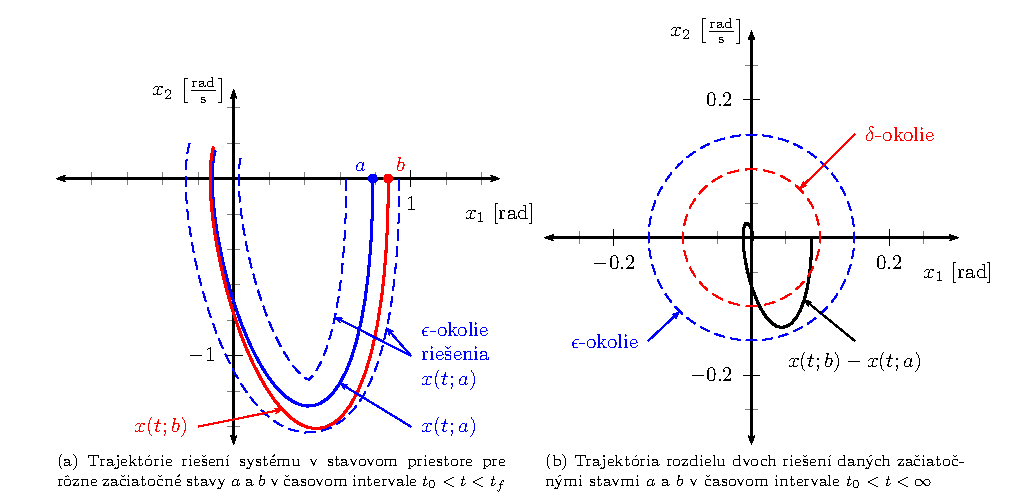
\includegraphics{Obr_LyapTraj.pdf}}

	\subfloat[]{\label{Trajektórie stavu kyvadla v stavovom priestore}}%
	\subfloat[]{\label{Trajektória rozdielu dvoch riešení daných začiatočnými stavmi }}%

		\vspace{-10mm}
	\caption{Ilustračný príklad k definícii stability riešenia systému}
	\label{Ilustračný príklad k definícii stability riešenia systému}
	%\vspace{-5mm}
\end{figure}







Ak je riešenie stabilné v zmysle Lyapunova, ale trajektórie okolitých riešení k nemu nekonvergujú, hovoríme, že riešenie je \emph{neutrálne stabilné}.

Riešenie $x(t;a)$ je \emph{asymptoticky stabilné} ak je stabilné v~zmysle Lyapunova a~zároveň $x(t;b) \to x(t;a)$ s~rastúcim časom $t \to \infty$ pri začiatočnom stave $b$, ktorý je dostatočne blízko stavu~$a$.

Veľmi dôležitým špeciálnym prípadom je ak pre skúmané riešenie platí $x(t;a) = x_e$. Potom nehovoríme o stabilite riešenia ale o~\emph{stabilite stacionárneho bodu}. Príkladom asymptoticky stabilného stacionárneho bodu sú body
\begin{align*}
	x_{e_{-2}} =
	\begin{bmatrix}
		-2\pi \\ 0
	\end{bmatrix},
	\quad
	x_{e_{0}} =
	\begin{bmatrix}
		0 \\ 0
	\end{bmatrix},
	\quad
	\text{a}
	\quad
	x_{e_{2}} =
	\begin{bmatrix}
		2 \pi \\ 0
	\end{bmatrix}
\end{align*}
na Obr.~\ref{Fázový portrét kyvadla}, vidíme, že ak začíname blízko asymptoticky stabilného stacionárneho bodu, s narastajúcim časom sa k nemu približujeme.

Riešenie $x(t;a)$ je \emph{nestabilné} ak nie je stabilné. Konkrétnejšie, hovoríme, že riešenie $x(t;a)$ je nestabilné ak pre akékoľvek dané $\epsilon > 0$ neexistuje $\delta > 0$ taká, že ak $\left\| b - a \right\| < \delta \; \text{potom} \; \left\| x(t;b) - x(t;a) \right\| < \epsilon, \; \forall \, t>0$. Príkladom nestabilného stacionárneho bodu sú body
\begin{align*}
	x_{e_{-1}} =
	\begin{bmatrix}
		-\pi \\ 0
	\end{bmatrix},
	\quad
	\text{a}
	\quad
	x_{e_{1}} =
	\begin{bmatrix}
		\pi \\ 0
	\end{bmatrix}
\end{align*}
na Obr.~\ref{Fázový portrét kyvadla}.

Predchádzajúce definície nezohľadňujú oblasť, na ktorej môžu byť použité. Presnejšie je definovať riešenie ako \emph{lokálne stabilné} (alebo \emph{lokálne asymptoticky stabilné}) ak je stabilné pre všetky začiatočné stavy $x \in B_r(a)$, kde $B_r(a) = \left\{ x \, : \, \| x - a \| < r \right\}$ je oblasť s polomerom $r > 0$ okolo bodu $a$. Riešenie je \emph{globálne stabilné} ak je stabilné pre všetky $r > 0$.



% \begin{center}

%     % \vbox{%
%     % \makebox[\textwidth][c]{%
%     % 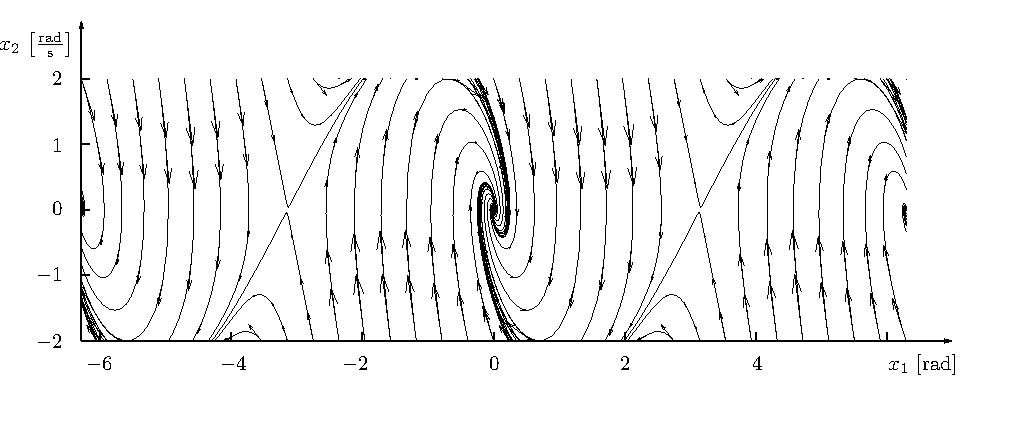
\includegraphics{Obr_KyvadloFazPortret.pdf}
%     % }

%     \subfloat[Fázový portrét nelineárneho modelu kyvadla]{%\label{Trajektórie stavu kyvadla v stavovom priestore}%
%     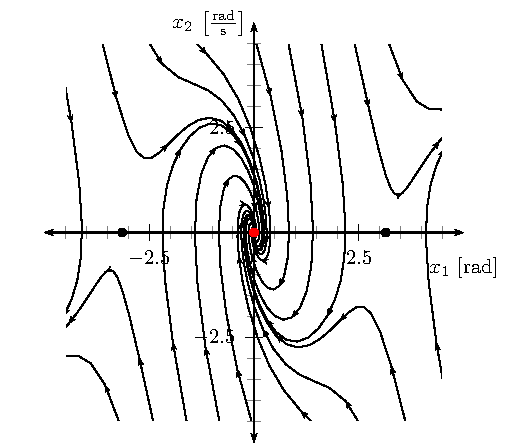
\includegraphics{Obr_FazPorNelin.pdf}
% }
% \hspace{1cm}
% \subfloat[Fázový portrét lineárneho modelu kyvadla]{%\label{Trajektórie stavu kyvadla v stavovom priestore}%
%     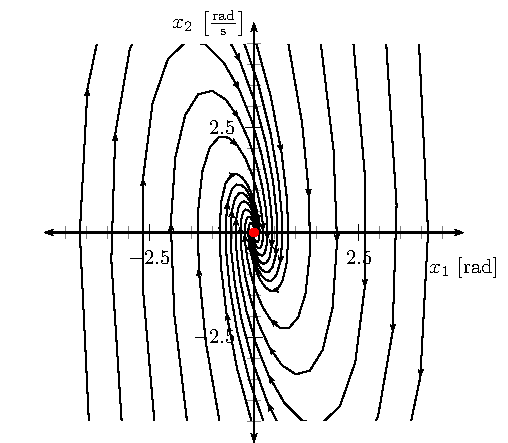
\includegraphics{Obr_FazPorLin.pdf}
% }

%     % \vspace{-6pt}

%     % \figcaption{Fázový portrét kyvadla (obrázok vytvorený v Matlabe, viď text pre zdrojový kód)}
%     % \label{Fázový portrét kyvadla}
%     }

% \end{center}




\begin{figure}[t]
	\centering

    \makebox[\textwidth][c]{%
	\subfloat[Fázový portrét nelineárneho modelu kyvadla]{%\label{Trajektórie stavu kyvadla v stavovom priestore}%
		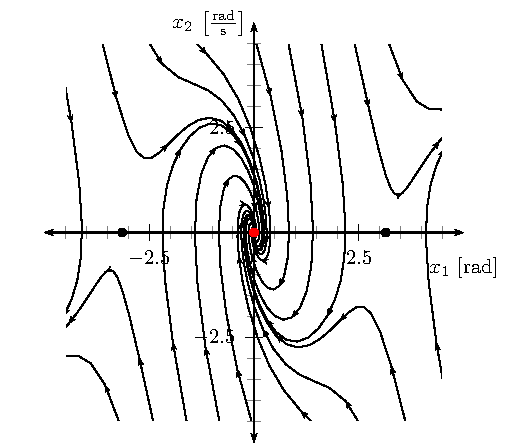
\includegraphics{Obr_FazPorNelin.pdf}
	}
	% \hspace{1cm}
	\subfloat[Fázový portrét lineárneho modelu kyvadla]{%\label{Trajektórie stavu kyvadla v stavovom priestore}%
		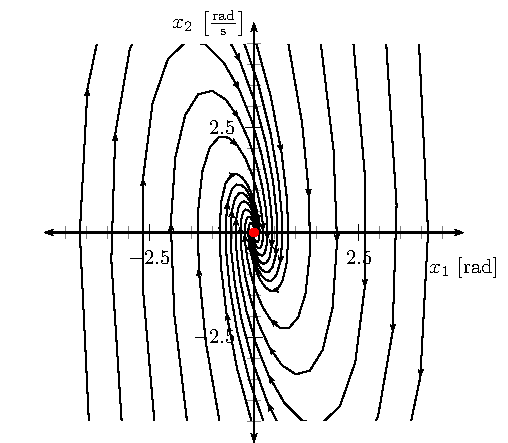
\includegraphics{Obr_FazPorLin.pdf}
	}
    }

	\caption{Porovnanie fázových portrétov nelineárneho systému a jeho linearizovanej aproximácie}
	\label{Porovnanie fázových portrétov nelineárneho systému a jeho linearizovanej aproximácie}
\end{figure}













\subsection{Stabilita lineárnych dynamických systémov}


Lineárny dynamický systém má tvar
\begin{equation}
	\dot{x} = A x, \quad x(0) = x_0
\end{equation}
kde $A \in \mathbb{R}^{n\times n}$ je štvorcová matica. Začiatok stavového priestoru je vždy stacionárnym bodom lineárneho systému a stabilita tohto stacionárneho bodu môže byť určená pomocou vlastných čísel matice $A$.

Vlastné čísla $\lambda(A)$ sú korene \emph{charakteristického polynómu} systému $\det(sI - A)$, kde $s \in \mathbb{C}$ je komplexná premenná a $I$ je jednotková matica. Konkrétne vlastné číslo ($i$-te vlastné číslo) označujeme $\lambda_i$, pričom $\lambda_i \in \lambda(A)$.
%Vo všeobecnosti je vlastné číslo matice $A$ $\lambda_i$ komplexné číslo a keď $A$ obsahuje len reálne čísla potom aj komlexne združené $\lambda_i^*$ je tiež vlastným číslom matice~$A$.

Pre lineárny systém stabilita stacionárneho bodu (ako veľmi dôležitého špeciálneho prípadu spomedzi všetkých riešení) závisí len od matice $A$, čo znamená, že stabilita je vlastnosť systému. Pre lineárny systém preto hovoríme o stabilite systému namiesto o~stabilite konkrétneho riešenia alebo ekvilibria.

Stabilitu lineárneho systému možno zhrnúť do jednej vety:

{ \it
\noindent
Systém
\begin{equation*}
	\dot{x} = A x
\end{equation*}
je asymptoticky stabilný vtedy a len vtedy keď reálne časti všetkých vlastných čísel matice $A$ sú záporné a systém je nestabilný keď aspoň jedno vlastné číslo matice $A$ má kladnú reálnu časť.
}



























\section{Otázky a úlohy}

\begin{enumerate}[leftmargin=0pt, labelsep=3mm, itemsep=0pt]

    
    \item Vysvetlite pojem \emph{prevodová charakteristika systému}.

    \item Ako sa nazýva vzájomná závislosť medzi ustálenými hodnotami výstupného signálu systému a ustálenými hodnotami vstupného signálu?

    \item Čo určuje sklon prevodovej charakteristiky?


    \item Vysvetlite pojem \emph{prechodová charakteristika systému}.

    \item Ako sa nazýva časový priebeh výstupného signálu systému po skokovej zmene vstupného signálu s jednotkovou veľkosťou?

    \item Majme homogénny dynamický systém daný rovnicou $ \dot x(t) = A x(t) $, kde $x(t) \in \mathbb R^n$ je vektor signálov. Určte ekvilibrium systému (ustálený stav) a~uveďte nutnú a~postačujúcu podmienku pre stabilitu ekvilibria.



\end{enumerate}







% \printbibliography[title={Literatúra}]





\end{document}
